\chapter[Metodologia]{Metodologia}

\section{Gerenciamento}

\subsection{Termo de Abertura do Projeto (TAP)}

O termo de abertura do projeto é essencial para que se documente de forma clara o atual cenário e o que será realizado no projeto, bem como ter noção de planejamento quanto a prazo e custos. O termo de abertura do projeto referente a esse trabalho se encontra disponível no anexo A.

\subsection{Estrutura Analítica do Projeto (EAP)}

A estrutura analítica do projeto possibilita uma visão geral das atividades que serão realizadas ao longo do projeto. Dessa forma, a EAP deste trabalho foi elaborada levando em conta os prazos de entregas, e a separação das macro atividades, ou subsistemas, e das micro atividades. Ela está disponível abaixo:

\begin{figure}[h]
	\centering
	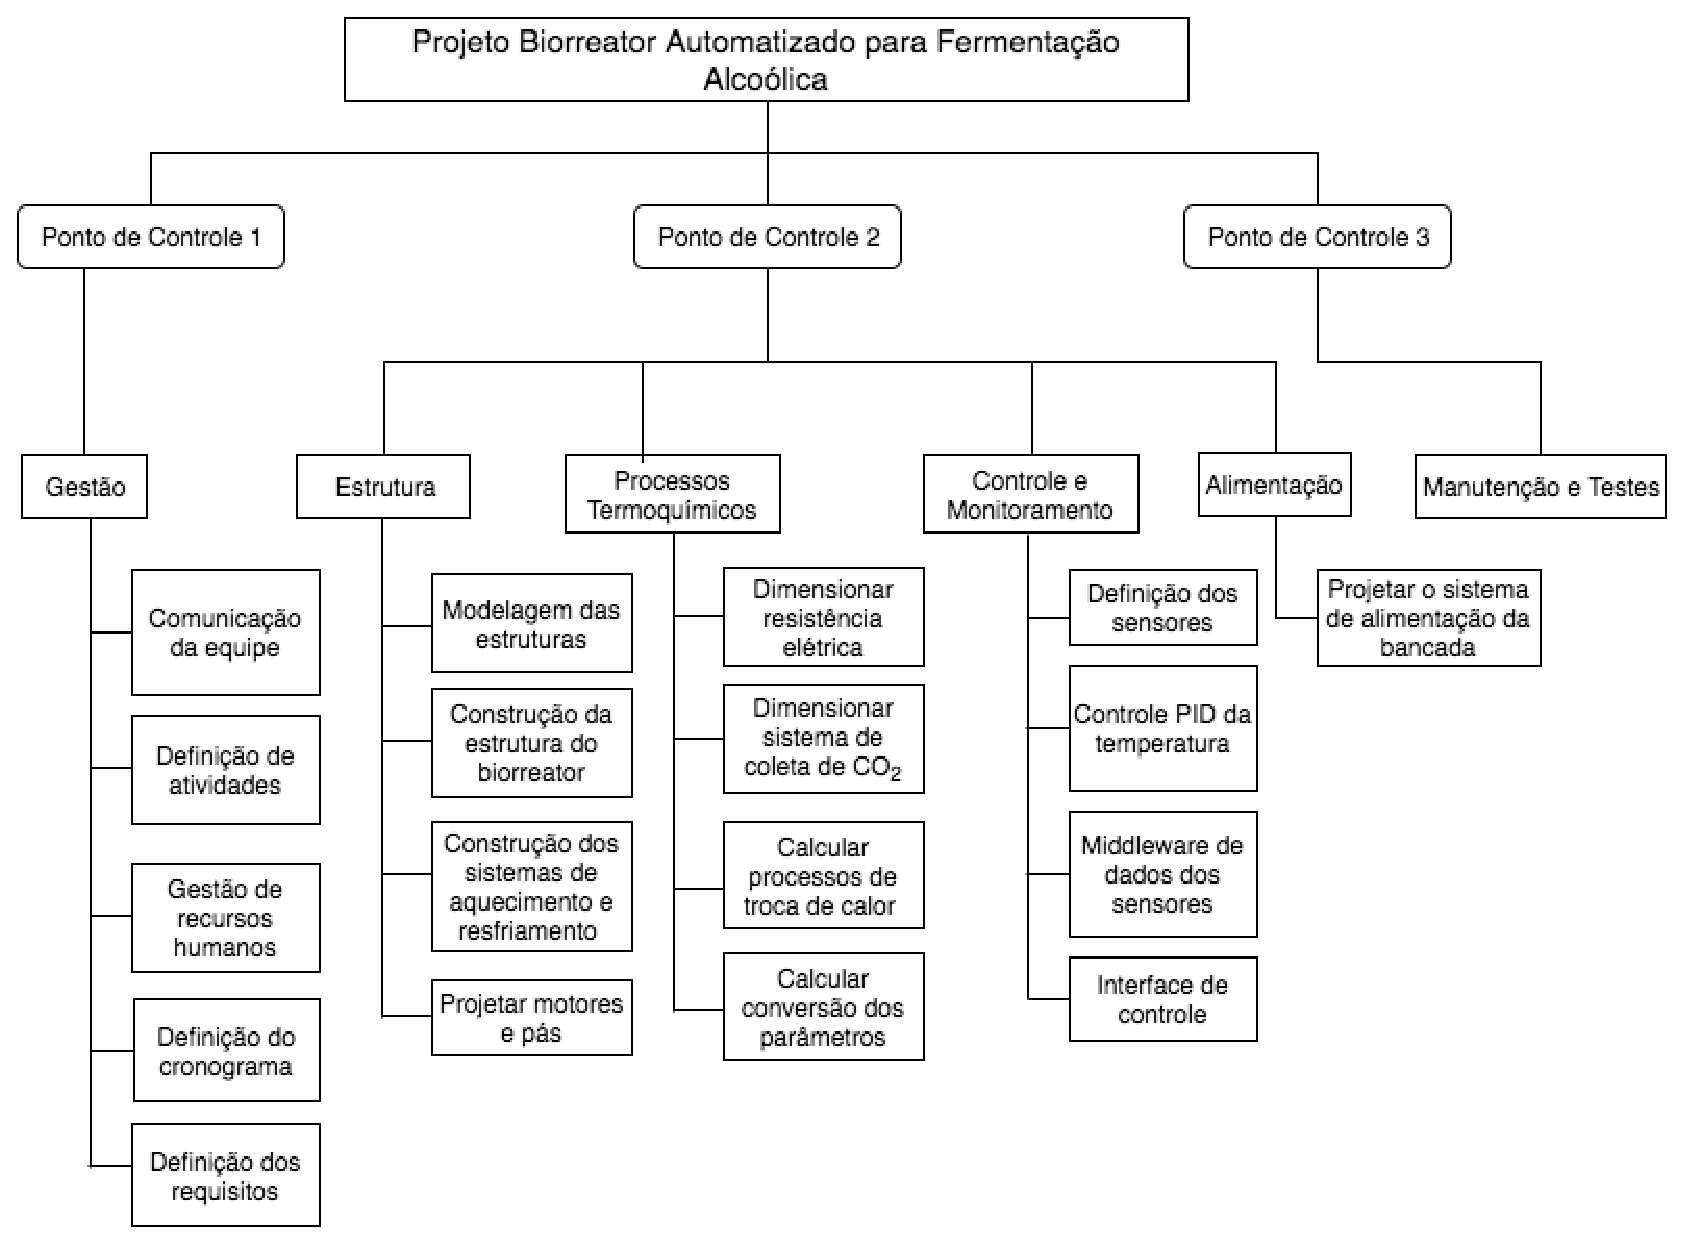
\includegraphics[keepaspectratio=true,scale=0.8, width=\textwidth]{figuras/eap.eps}
	\caption{Estrutura Analítica do Projeto}
	\label{eap}
\end{figure}

\subsection{Tempo}

Baseado nos prazos de entrega nos pontos de controle, foi feito o seguinte cronograma de atividades:

\subsection{Custos}

O gerenciamento dos custos do projeto inclui os processos envolvidos em planejamento, estimativas, orçamentos, financiamentos, gerenciamento e controle dos custos, de modo que o projeto possa ser terminado dentro do orçamento aprovado possuindo foco no custo dos recursos necessários para completar as atividades do projeto.

O gerenciamento dos custos projeto deve considerar também o efeito das decisões de projeto no custo recorrente subsequente do uso, manutenção e suporte do produto, serviço ou resultado do projeto, neste caso ficando limitado a opção da equipe quanto a continuar disponibilizando e oferecendo suporte ao produto final.

A tabela abaixo representa os custos estimados dos materiais selecionados para o desenvolvimento do projeto:

\begin{table}[h]
\centering
\caption{Tabela de custos do projeto}
\resizebox{\textwidth}{!} {
\label{table1}
\begin{tabular}{ll|l|}
\hline
\multicolumn{1}{|l|}{Area}                     & Material                                                                                    & Custo              \\ \hline
\multicolumn{1}{|l|}{ESTRUTURA}                & Conformação mecânica (calandragem) cilíndrica, cônica para aço inoxidável e flange (1,5 mm) & R\$332,00          \\ \hline
\multicolumn{1}{|l|}{}                         & Soldagem inox                                                                               & R\$300,00          \\ \hline
\multicolumn{1}{|l|}{}                         & Tubo de Suporte                                                                             & R\$130,00          \\ \hline
\multicolumn{1}{|l|}{}                         & Tampa flangeada (3 mm)                                                                      & R\$ 120,00         \\ \hline
\multicolumn{1}{|l|}{}                         & Válvula de alívio de pressão                                                                & R\$ 11,15          \\ \hline
\multicolumn{1}{|l|}{}                         & Manômetro                                                                                   & R\$ 37,00          \\ \hline
\multicolumn{1}{|l|}{}                         & 11 Anéis de vedação em silicone (espude)                                                    & R\$ 20,00          \\ \hline
\multicolumn{1}{|l|}{}                         & 2 Torneiras                                                                                 & R\$ 20,00          \\ \hline
\multicolumn{1}{|l|}{}                         & Rotor e Pás                                                                                 & R\$ 50,00          \\ \hline
\multicolumn{1}{|l|}{}                         & Motor                                                                                       & R\$ 300,00         \\ \hline
\multicolumn{1}{|l|}{}                         & Rolamentos                                                                                  & R\$ 10,00          \\ \hline
\multicolumn{1}{|l|}{CONTROLE E MONITORAMENTO} & Sensor Ultrassônico HC-SR04                                                                 & R\$ 15,00          \\ \hline
\multicolumn{1}{|l|}{}                         & 2 Sensores DS18B20 para temperatura                                                         & R\$ 20,40          \\ \hline
\multicolumn{1}{|l|}{}                         & 2 sensores MPX5700DP                                                                        & R\$ 123,00         \\ \hline
\multicolumn{1}{|l|}{}                         & Gravity Analog pH Meter Kit                                                                 & R\$ 147,00         \\ \hline
\multicolumn{1}{|l|}{}                         & Motor de Passo 28BYJ-48 + Driver ULN2003                                                    & R\$ 20,00          \\ \hline
\multicolumn{1}{|l|}{}                         & Conversor A/D ADS1115                                                                       & R\$ 24,00          \\ \hline
\multicolumn{1}{|l|}{}                         & Raspberry PI 3                                                                              & R\$ 200,00         \\ \hline
\multicolumn{1}{|l|}{PROCESSOS TERMOQUÍMICOS}  & Resistência elétrica 5000 W 220 V                                                           & R\$ 100,00         \\ \hline
\multicolumn{1}{|l|}{}                         & Bomba de circulação 220 V                                                                   & R\$ 250,00         \\ \hline
\multicolumn{1}{|l|}{}                         & Mangueira de silicone                                                                       & R\$ 14,00/m        \\ \hline
\multicolumn{1}{|l|}{}                         & Alga chaetomorpha                                                                           & R\$ 34,90          \\ \hline
\multicolumn{1}{|l|}{}                         & Válvula de esfera para gás borboleta fêmea                                                  & R\$ 30,00          \\ \hline
\multicolumn{1}{|l|}{ALIMENTAÇÃO}              & Cabo de Força 3m                                                                            & R\$ 25,00          \\ \hline
                                               &                                                                                             & TOTAL: R\$2.419,55 \\ \cline{3-3}
\end{tabular}
}
\end{table}

\subsection{Alocação de recursos humanos}

A equipe do projeto é formada por 12 membros que foram divididos de acordo com as macro atividades que serão realizadas. Em cada uma delas foi escolhido um membro líder responsável pela supervisão das atividades. Além disso, foi escolhido um líder geral, o gerente do projeto, responsável pela integração de todas as partes do mesmo, e um outro gerente responsável pelo controle de qualidade das atividades. Abaixo se tem a relação esquemática da divisão adotada.

\begin{figure}[h]
	\centering
	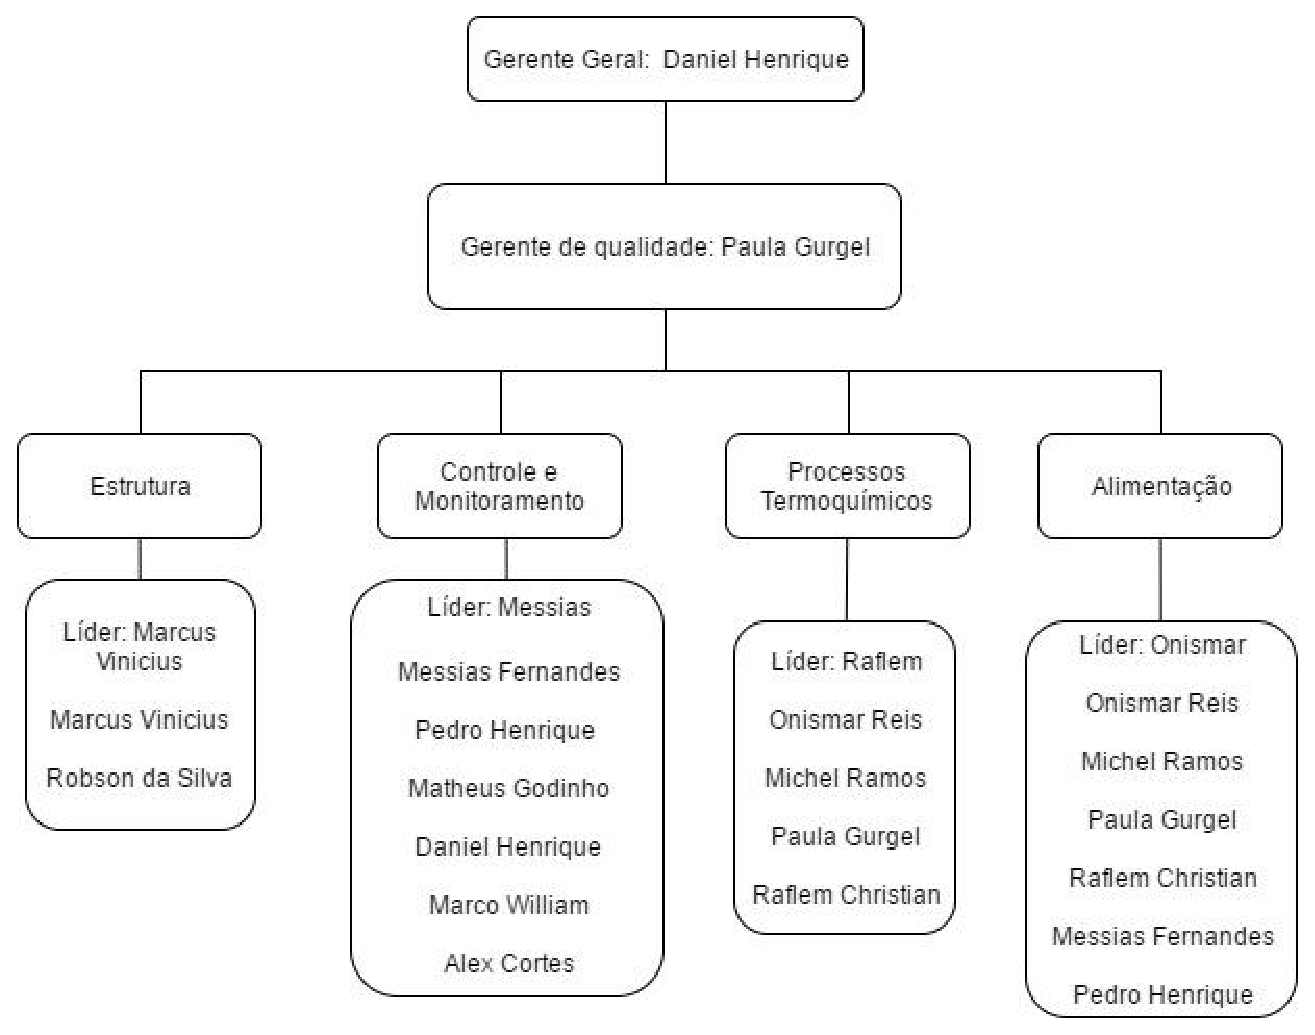
\includegraphics[keepaspectratio=true,scale=0.5]{figuras/divisao.eps}
	\caption{Divisão de frentes de trabalho e gerentes do projeto}
	\label{divisao}
\end{figure}

\subsection{Riscos}

Um plano de gerenciamento de riscos é necessário para calcular o impacto dos riscos no projeto e medidas de contingência para o controles dos mesmos. O plano de gerenciamento de riscos está disponível no anexo A.

\subsection{Requisitos}

A partir da concepção e validação do solucionamento do sistema, os requisitos foram definidos a partir de cada subsistema deste presente projeto.

\begin{itemize}
\item O biorreator deverá ser capaz de aquecer e resfriar dentro da faixa de 0º a 100º Celsius.
\item Ter um sistema que seja capaz de coletar CO2.
\item O rotor do sistema deverá manter-se a uma velocidade constante e pré-determinada.
\item O biorreator deverá possuir dimensões capazes de acomodar os sensores e demais componentes internos definidos no projeto.
\item Quanto a estrutura do biorreator, deverá possuir em sua composição, material favorável quanto a assepsia que o sistema necessita.
\item A dimensão da estrutura do biorreator deverá estar de conformidade com um equipamento de bancada de um laboratório.
\item O biorreator deverá possuir um motor, conectado ao seu rotor, para que a agitação mecânica seja realizada.
\item O biorreator deverá ser automatizado o suficiente para realizar a coleta de dados dos principais parâmetros e gerar gráficos.
\item O biorreator deverá realizar a leitura de dados referente a temperatura, pH, densidade e volume.
\item O biorreator deverá possuir um compartimento, especificamente de açúcar, para se auto-alimentar, quando necessário.
\item O biorreator deverá possuir uma válvula para realizar a coleta da levedura.
\item O biorreator deverá possuir uma válvula de precaução em caso de um aumento de pressão.
\item O biorreator deverá ter um sistema de aquecimento interligado a um controlador PID (Proporcional, Integral e derivativo).
\item Todo o sistema do biorreator deve estar conectado a um sistema de software e  hardware, que o usuário possa ver e controlar todos os parâmetros do mesmo.
\end{itemize}

\subsection{Controle e Monitoramento}

Dada a especificação do projeto, pretende-se realizar medições eletrônicas de valores de temperatura, densidade e potencial hidrogênico(pH). A partir, disso seria utilizado uma unidade microcontrolada para processamento de dados.

Com relação a unidade de controle e aquisição de dados para o monitoramento do sistema será atacado em duas frentes. A primeira solução adotada para este problema será usar uma \textit{Raspberry PI 3}, para realizar a aquisição e processamento de dados, para exercer essa atividade deve-se desenvolver uma biblioteca para cada sensor, com o auxílio de conversores analógicos/digitais para facilitar a recepção de dados pela Raspberry, essa solução pretende reduzir os itens envolvidos no projeto. Em paralelo será trabalhado uma solução alternativa, onde os dados enviados pelos sensores serão recebidos por um microcontrolador Arduino ATMEGA 238, e o dados serão processados e enviados para uma \textit{Raspberry PI 3}, através de um protocolo de comunicação \textit{UART}, para receber e realizar o processamento de dados.

\subsubsection{Medição de temperatura}

Para realizar medições de temperatura foi escolhido o sensor DS18B20, Com relação às suas especificações elétricas, este possui uma variação de tensão de alimentação nos seus pinos de -0.5 a +6V e a faixa de variação na escala de temperatura permite medições que variam de -55ºC a +125ºC. Esta escala de variação é adequada para a medição de valores de temperatura, já que o valor máximo para valores seria de aproximadamente 100ºC no interior do biorreator.

Sobre a precisão do componente, os valores de saída são discretizados na em 8 bits. Ou seja, os 180 valores possíveis de medição são exibidos com precisão de 0,703125ºC. O sensor além disso, possui características à prova de água, devido ao seu encapsulamento, o que facilita a imersão no interior do biorreator.

\begin{figure}[h]
	\centering
	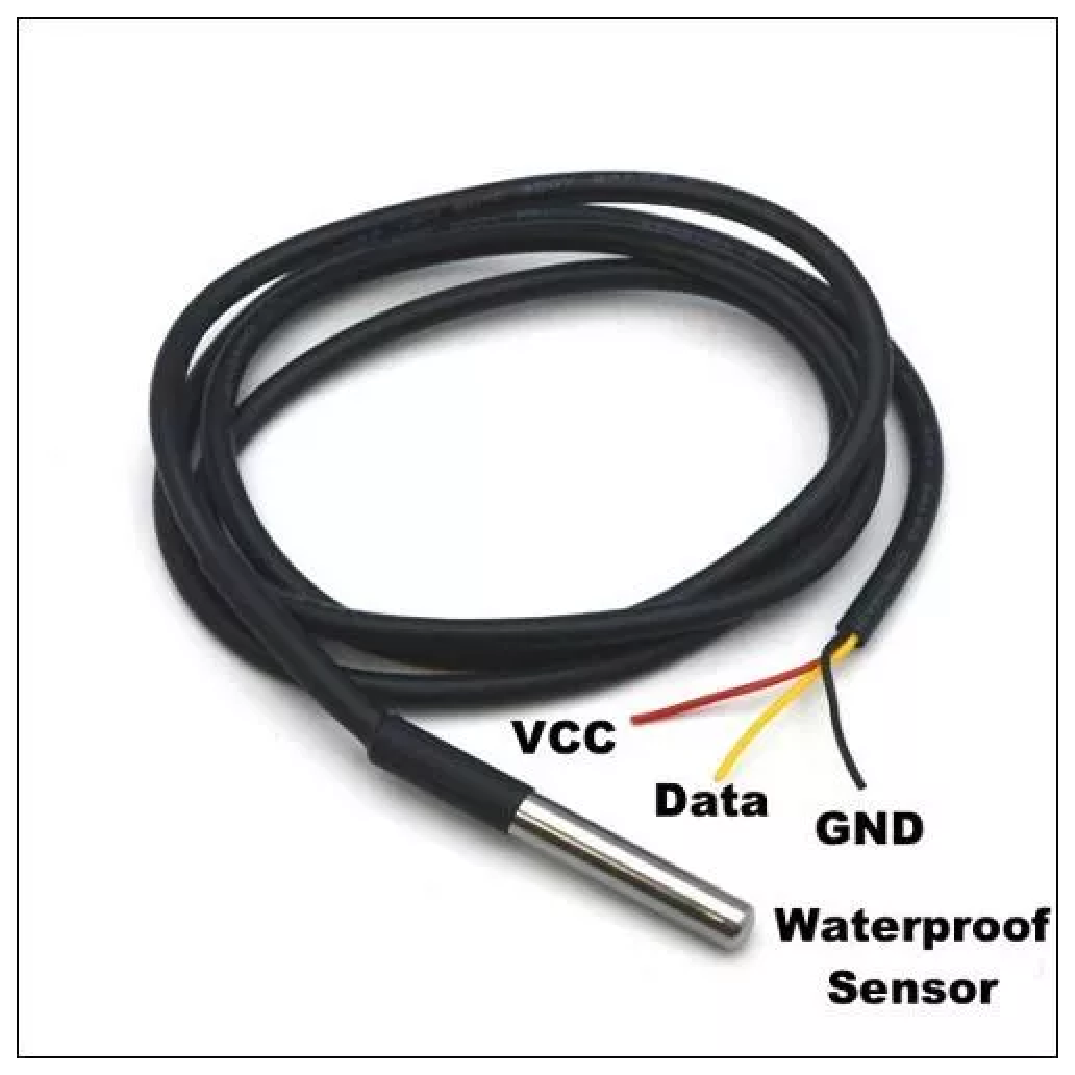
\includegraphics[keepaspectratio=true,scale=0.3]{figuras/probe.eps}
	\caption{Probe para imersão em fluidos}
	\label{probe}
\end{figure}

\subsubsection{Medição de densidade}

A definição da densidade no projeto \nocite{ADS1115} é um requisito para provar a funcionalidade do projeto, torna-se necessário a sua medição. Considerando que o uso de um sensor de densidade é inviável de medição, usa-se o princípio da medição de pressão diferencial para estimar o valor da densidade através da manipulação da equação de Bernoulli. A especificação da medição de densidade, torna-se necessário o uso de sensores de pressão aplicados em dois pontos distintos no interior do biorreator.

\begin{figure}[h]
	\centering
	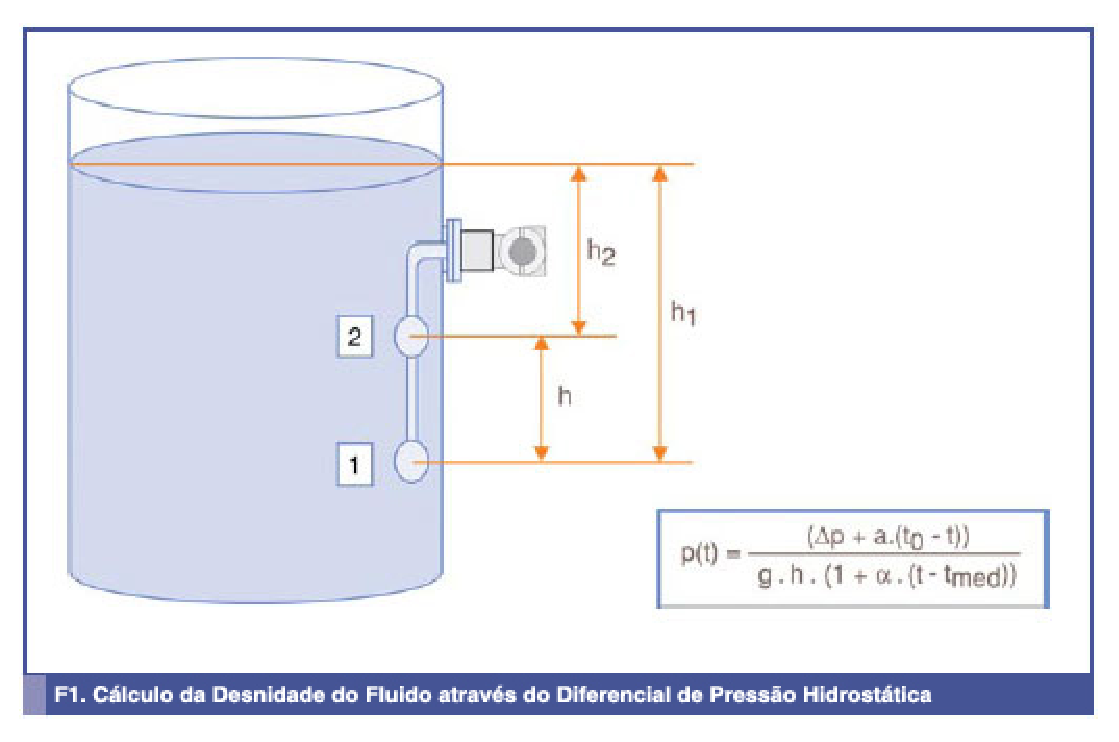
\includegraphics[keepaspectratio=true,scale=0.4]{figuras/densidade.eps}
	\caption{Modelo de cálculo da densidade de um fluido por pressão diferencial}
	\label{densidade}
\end{figure}

Com relação ao coeficientes e parâmetros matemáticos tem-se:

\begin{itemize}
\item \( \rho \): Densidade
\item t: Temperatura do processo
\item \( \Delta \)P: Diferença de Pressão
\item a: Coeficiente de compensação de temperatura no fluído
\item tZERO = Temperatura de Calibração do sensor
\item g: Aceleração da gravidade
\item h: Distância entre os pontos de medição
\item \( \alpha \): Coeficiente de dilatação do material da estrutura
\item tMED: Temperatura de medição nos pontos de medição
\end{itemize}

Dada tal necessidade adotou-se ao projeto o sensor MPX5700DP para medição de pressão sua especificações elétricas são:

\begin{itemize}
  \item Faixa de pressão operacional: 15kPa a 700kPa (0.15 ~ 6.9 atm);
  \item Tensão de alimentação: 5V;
  \item Nº de Pinos: 6;
  \item Pinos úteis: 3;
  \item Precisão: V/P: 6.4mV/kPa;
  \item Corrente de suprimento 7mA;
  \item Faixa de temperatura de operação: -40ºC a + 125ºC;
  \item Dimensões (CxLxA): ~29x37x8mm;
\end{itemize}

\subsubsection{Medição de Volume}

Tal componente utiliza sinais ultrassônicos para determinar a distância entre o sensor e um determinado obstáculo. De modo que no projeto em questão, será responsável por determinar a distância entre o sensor e o nível de açúcar presente na válvula, aferindo assim a quantidade de açúcar ali presente e retornando um dado para o servidor. Apresenta a seguinte tabela de especificações: \nocite{28BYJ-48}

\begin{table}[h]
\centering
\caption{Especificações técnicas Sensor HC-SR04}
\resizebox{\textwidth}{!} {
\label{table2}
\begin{tabular}{|l|l|}
\hline
Tensão de Funcionamento                      & 5 V – DC                                              \\ \hline
Corrente de Funcionamento                    & 15 mA                                                 \\ \hline
Frequência de Funcionamento                  & 40 KHz                                                \\ \hline
Intervalo máximo de verificação de distância & 4 m                                                   \\ \hline
Intervalo mínimo de verificação de distância & 2 cm                                                  \\ \hline
ngulo de Detecção                            & 15º                                                   \\ \hline
Sinal de Entrada Trigger                     & 10uS pulso TTL                                        \\ \hline
Sinal de Saída Echo                          & Entrada do sinal de nível TTL e da faixa de proporção \\ \hline
Dimensão                                     & 45-20-15 mm                                           \\ \hline
\end{tabular}
}
\end{table}

\begin{figure}[h]
	\centering
	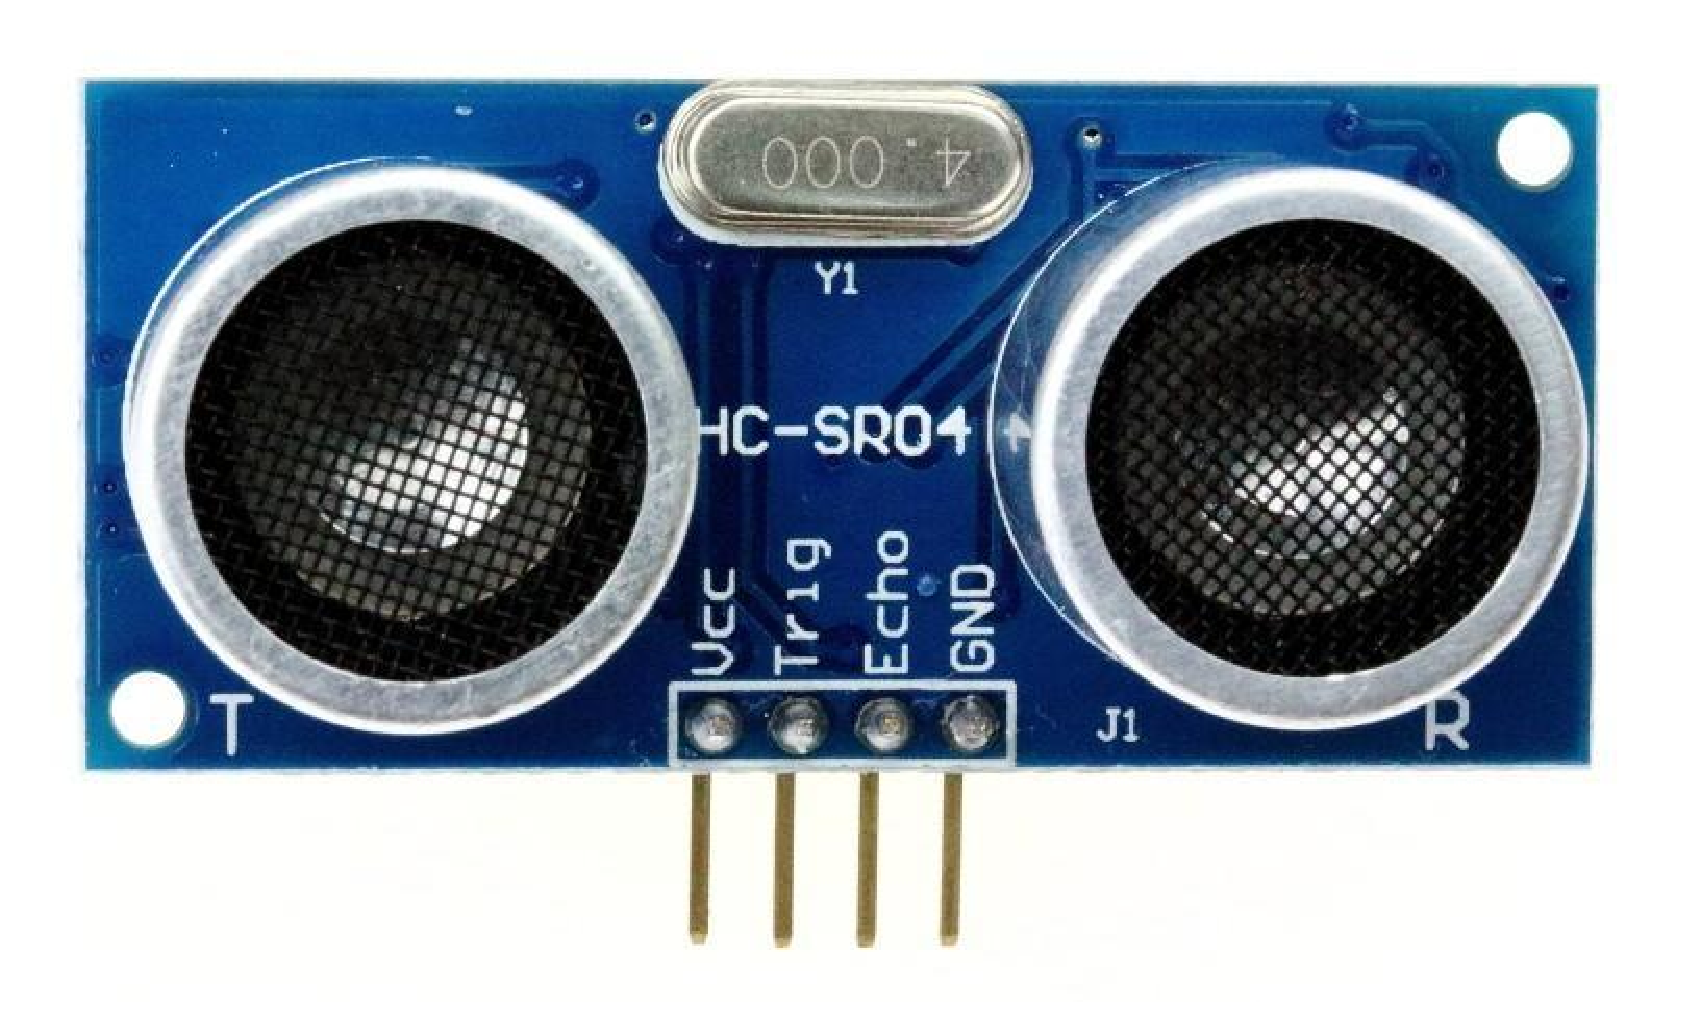
\includegraphics[keepaspectratio=true,scale=0.2]{figuras/sensor1.eps}
	\caption{Ilustração do Sensor HC-SR04}
	\label{sensor1}
\end{figure}

Assim como ilustrado pela imagem acima \nocite{MCP4725} o componente possui 4 pinos (Vcc, Trigger, Echo, GND), onde serão conectados de acordo com as especificações técnicas ditas anteriormente.

\subsubsection{Medição de pH}

  Com relação a especificação da medição de pH, torna-se necessário o uso do kit SKU: SEN0161 que é um kit integrado com um indicador de alimentação, um conector BNC e interface do sensor PH2.0. Segue abaixo a especificação: \nocite{HC-SR04}

\begin{itemize}
  \item Potência do módulo: 5.00V
  \item Tamanho da placa de circuito: 43mm x 32mm
  \item Faixa de medição do pH: 0-14
  \item Temperatura de medição: 0-60 ºC
  \item Precisão: +- 0.1pH (25 ºC)
  \item Tempo de resposta: <=   1min
  \item Sensor de pH com conector BNC
  \item Interface PH2.0 (patch de 3 pés)
  \item Potenciômetro de ajuste de ganho
  \item Indicador de energia LED
\end{itemize}

Calibração do Kit:

\begin{figure}[h]
	\centering
	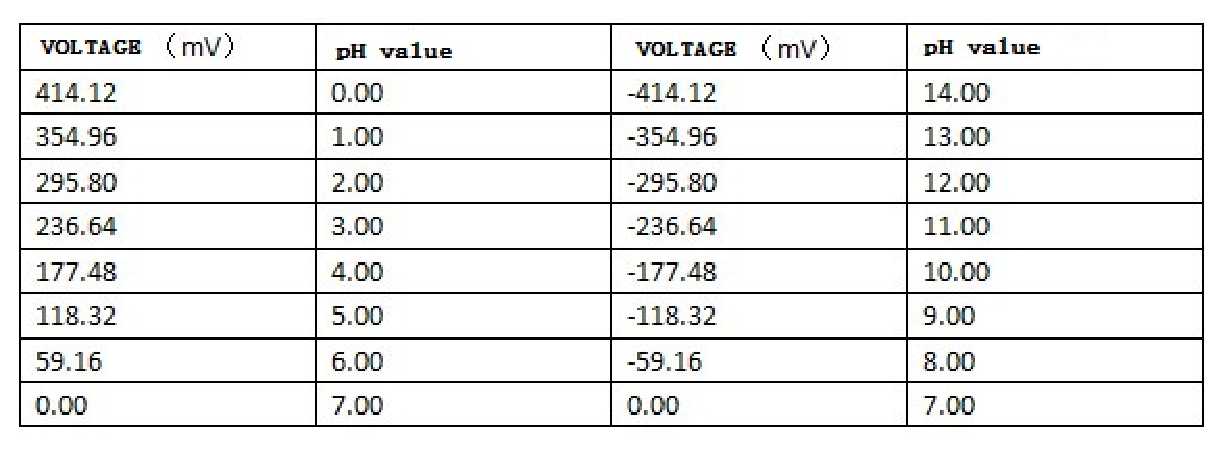
\includegraphics[keepaspectratio=true,scale=0.6]{figuras/ph.eps}
	\caption{Voltagem de Saída medida em relação ao pH}
	\label{ph}
\end{figure}

\begin{figure}[h]
	\centering
	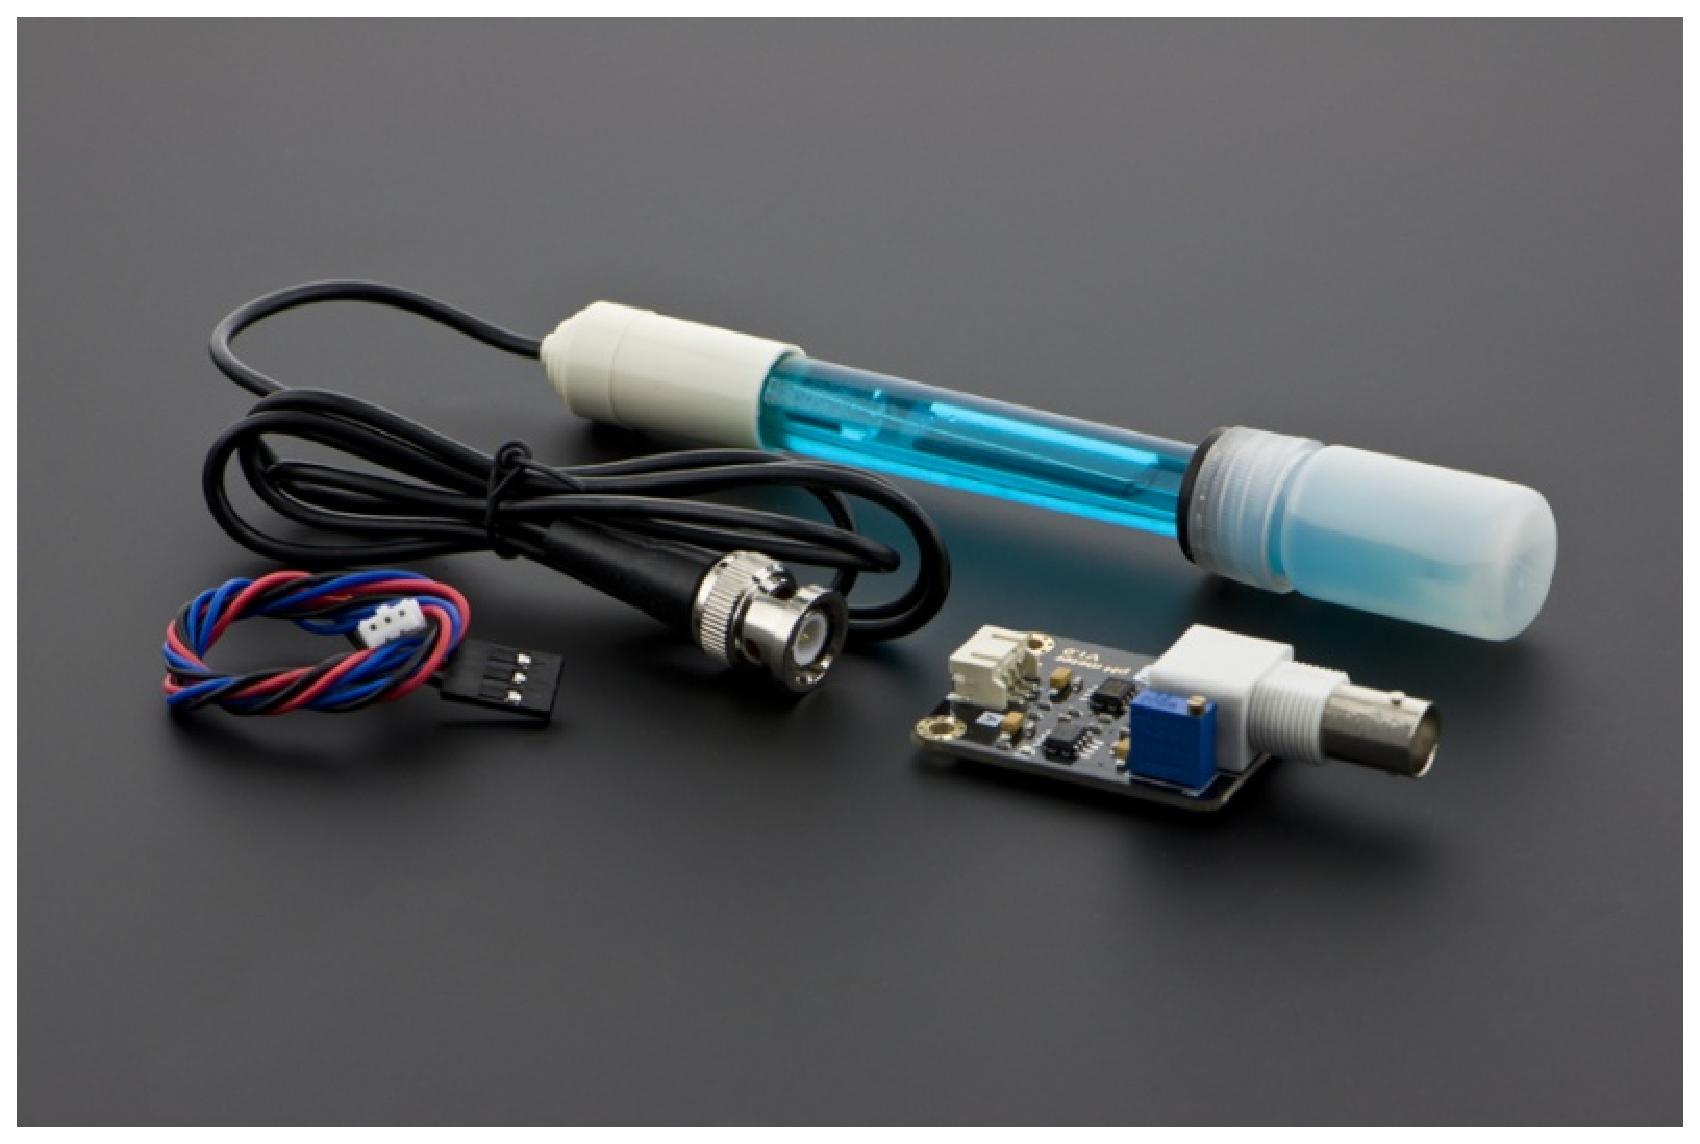
\includegraphics[keepaspectratio=true,scale=0.3]{figuras/sensorph.eps}
	\caption{Kit a ser adotado para medição de pH.}
	\label{sensorph}
\end{figure}

\subsubsection{Válvula de Liberação de açúcar}

Para realizar a liberação de açúcar em tempos contínuos será utilizado um motor de passos para habilitar o despejo de açúcar na função de válvula. Para isso foi escolhido o componente Motor de Passo 28BYJ-48 + Driver ULN2003. Tal componente utiliza conversão de \nocite{ADS1115} tensão em movimentos rotacionais, de modo a codificar o mesmo de modo a parar em posições específicas. De modo que este elemento será utilizado para o controle da válvula de depósito de açúcar, que quando acionado dá-se o passo necessário para liberação da quantidade de açúcar necessária para dentro do Biorreator. Já o Driver, é um sistema vendido juntamente ao motor, qual permite tal codificação de controle. Observa-se as seguintes especificações: \nocite{SEN0161}

\begin{table}[h]
\centering
\caption{Especificação Motor de Passo 28BYJ-48}
\label{table3}
\begin{tabular}{|l|l|}
\hline
Tensão de Funcionamento & 5 V – DC   \\ \hline
Número de Fases         & 4          \\ \hline
Número de Vias          & 5          \\ \hline
Passos por Volta        & 64         \\ \hline
Torque máximo           & 2.2 Kgf.cm \\ \hline
Ângulo por passo        & 5.625º/64  \\ \hline
Frequência              & 100 Hz     \\ \hline
Diâmetro do Eixo        & 5 mm       \\ \hline
Peso                    & 40 g       \\ \hline
\end{tabular}
\end{table}

\begin{figure}[h]
	\centering
	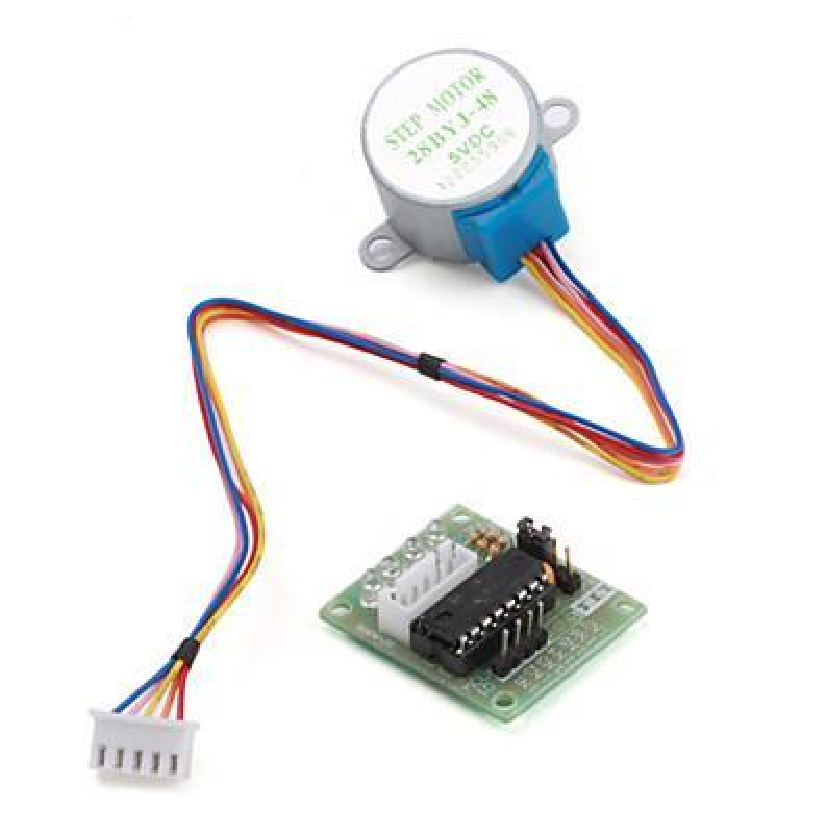
\includegraphics[keepaspectratio=true,scale=0.4]{figuras/sensor2.eps}
	\caption{Motor de Passo 28BYJ-48}
	\label{sensor2}
\end{figure}

\subsubsection{Conversor A/D ADS1115}

Tal componente realiza a conversão de tensão Analógica para Digital. Onde, na aplicação em estudo, será responsável por receber os sinais dos sensores em tensão analógica, converter para digital e encaminhar para o microcontrolador \textit{Raspberry}. Observa-se as seguintes especificações: \nocite{MPX5700}

\begin{table}[h]
\centering
\caption{Especificações Conversor ADS1115}
\label{table4}
\begin{tabular}{|l|l|}
\hline
Tensão de Funcionamento    & 2.0 – 5.5 V (DC) \\ \hline
Canais                     & 4                \\ \hline
Resolução                  & 16 bits          \\ \hline
Frequência de operação SLC & 0.1 -3.4 MHz     \\ \hline
Taxa de Dados              & 8 – 860 SPS      \\ \hline
Dimensões                  & 2 x 1.5 x 0.4 mm \\ \hline
\end{tabular}
\end{table}

\begin{figure}[h]
	\centering
	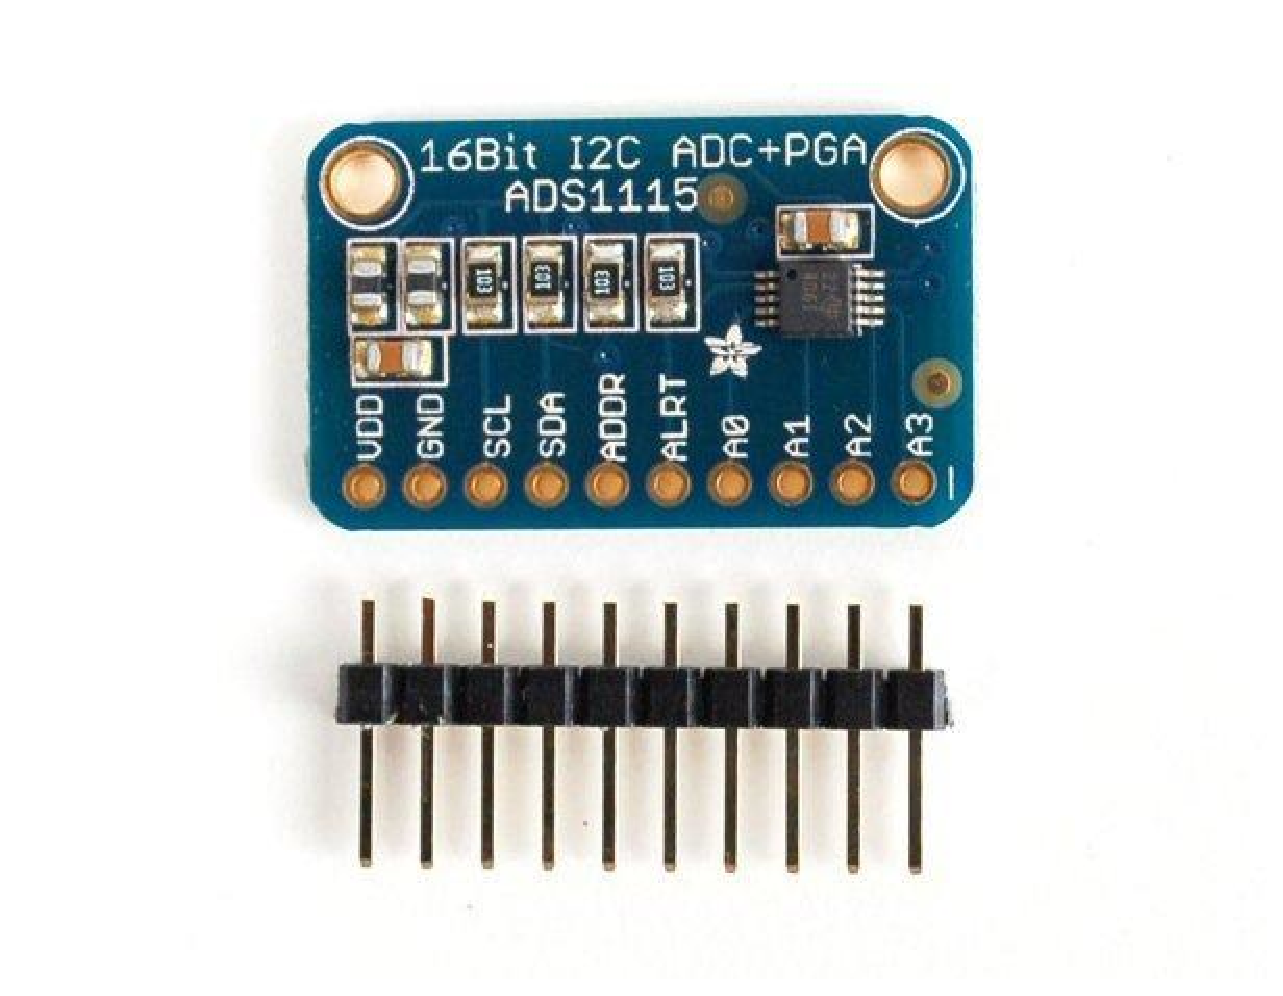
\includegraphics[keepaspectratio=true,scale=0.3]{figuras/sensor3.eps}
	\caption{Conversor ADS1115}
	\label{sensor3}
\end{figure}

\subsubsection{Conversor D/A MCP4725}

Tal componente realiza a conversão de tensão Digital para Analógico. Onde, na aplicação em estudo, será responsável por converter os sinais do cliente/usuário lançados pelo app em tensão digital, quais passam pelo servidor  microcontrolador \textit{Raspberry}, chegam no conversor em questão e são encaminhados para os Atuadores. Observa-se as seguintes especificações:\nocite{ds18b20}

\begin{table}[h]
\centering
\caption{Especificações técnicas Conversor D/A MCP4725}
\label{table5}
\begin{tabular}{|l|l|}
\hline
Tensão de Funcionamento & 2.7 – 5.5 V (DC) \\ \hline
Canais                  & 1                \\ \hline
Resolução               & 12 bits          \\ \hline
\end{tabular}
\end{table}

\begin{figure}[h]
	\centering
	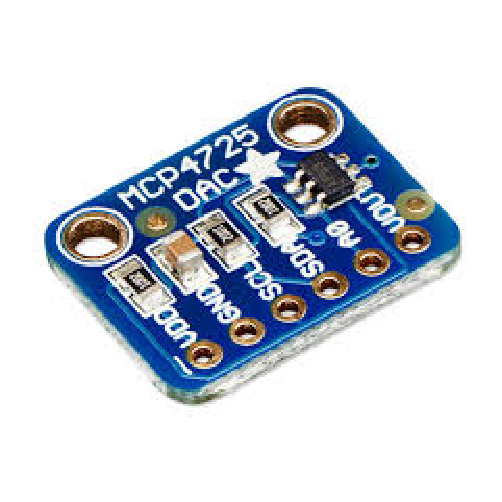
\includegraphics[keepaspectratio=true,scale=0.5]{figuras/sensor4.eps}
	\caption{Conversor D/A MCP4725}
	\label{sensor4}
\end{figure}

\subsubsection{Aplicativo}

Os requisitos do aplicativo foram definidos em formato de \textit{user stories}, identificadas como USXX sendo XX o número da \textit{user story}.

\subsubsubsection{US01}

Eu como usuário desejo visualizar os dados dos sensores para ter um monitoramento da fermentação no biorreator.

Critérios de aceitação:
\begin{itemize}
  \item Dados em forma de gráficos
  \item Gráficos gerados em tempo real
  \item Monitorar sensor de ph
  \item Monitorar sensor de densidade
  \item Monitorar sensor de temperatura
\end{itemize}

Tarefas:
\begin{itemize}
  \item Criar endpoint que disponibiliza os dados pela api
  \item Criar front-end no app para os gráficos
  \item Criar comunicação api-app para capturar os dados
\end{itemize}

\subsubsubsection{US02}

Eu como usuário desejo controlar a temperatura do biorreator para que a fermentação ocorra corretamente do início ao fim.

Critérios de aceitação:
\begin{itemize}
  \item Inserir a quantidade de graus desejada
\end{itemize}

Tarefas:
\begin{itemize}
  \item Criar endpoint para receber dados na api
  \item Criar front-end do app para receber a temperatura
  \item Criar comunicação app-api para enviar dados
\end{itemize}

\subsubsubsection{US03}

Eu como usuário desejo criar uma fermentação para poder diferenciar os dados do aplicativo por fermentação

Critérios de aceitação:
\begin{itemize}
  \item Título
  \item Data de início
  \item Data de término
\end{itemize}

Tarefas:
\begin{itemize}
  \item Criar endpoint para salvar fermentação na api
  \item Criar front-end da criação de fermentação no app
  \item Criar comunicação app-api para salvar fermentação
\end{itemize}

\subsubsubsection{US04}

Eu como usuário desejo controlar a quantidade de açúcar do biorreator para ter um controle do pH.

Critérios de aceitação:
\begin{itemize}
  \item Quantidade de rotações que o motor vai executar
\end{itemize}

Tarefas:
\begin{itemize}
  \item Criar endpoint para receber os dados do controle de açúcar
  \item Criar front-end que recebe a quantidade de rotações do motor no app
  \item Criar comunicação app-api para enviar os dados de quantidade de rotações
\end{itemize}

\subsubsubsection{US05}

Eu como usuário desejo gerar um relatório sobre uma determinada fermentação para ver o que aconteceu de certo e errado.

Critérios de aceitação:
\begin{itemize}
  \item Gerar relatório em pdf
  \item Gerar relatório no próprio aplicativo
\end{itemize}

Tarefas:
\begin{itemize}
  \item Gerar endpoint que enviará todos os dados do relatório
  \item Gerar estrutura do pdf
  \item Fazer front-end do relatório no app
  \item Fazer comunicação de dados app-api
  \item Gerar pdf
\end{itemize}

\subsubsubsection{US06}

Eu como usuário desejo receber notificações com os status do biorreator para monitorar sem o aplicativo estar aberto.

Critérios de aceitação:
\begin{itemize}
  \item Push notification quando finalizar o processo
  \item Push notification quando algum sensor apresentar dados suspeitos
\end{itemize}

Tarefas:
\begin{itemize}
  \item Configurar serviço de push notification na api
  \item Configurar serviço de push notification no app
  \item Criar momentos de envio da push notification na api
\end{itemize}

\section{Especificação do biorreator}

\subsection{Estrutura}

O intuito inicial do projeto seria em adotar normas para vasos de pressão, sendo estas a Norma Regulamentadora 13, de aplicação nacional, e a norma regulamentada pela ASME \textit{(American Society of Mechanical Engineers)}, porém devido a falta de recursos financeiros para seguí-los, os docentes sugeriram formular o projeto como um protótipo. O protótipo foi formulado no CATIA como prévia para fabricação, sendo passível de alterações futuras.

O material adotado no projeto para o desenvolvimento do alicerce do biorreator foi o aço inoxidável 304 devido a diversos motivos, como o alto grau de pureza presente na peça em relação aos demais aços, sendo que esta pureza se torna necessária pertinente a fermentação que ocorrerá, não sendo possível a realização com elementos contaminantes na reação, outro fato se dá a alta condução térmica, aperfeiçoando a troca de calor para uma maior eficiência na transferência de calor do sistema.

As chapas metálicas serão adquiridas e remetidas para calandragem, onde tomarão forma cônica e cilíndrica para a adequação  ao projeto. O fundo do tanque com formato esférico foi cogitado, mas diante a dificuldade em conformar a peça tornou-se impraticável sua produção.

As figuras abaixo ilustram a modelagem realizada para ter como ponto de partida o desenvolvimento estrutural do biorreator.

\begin{figure}[h]
	\centering
	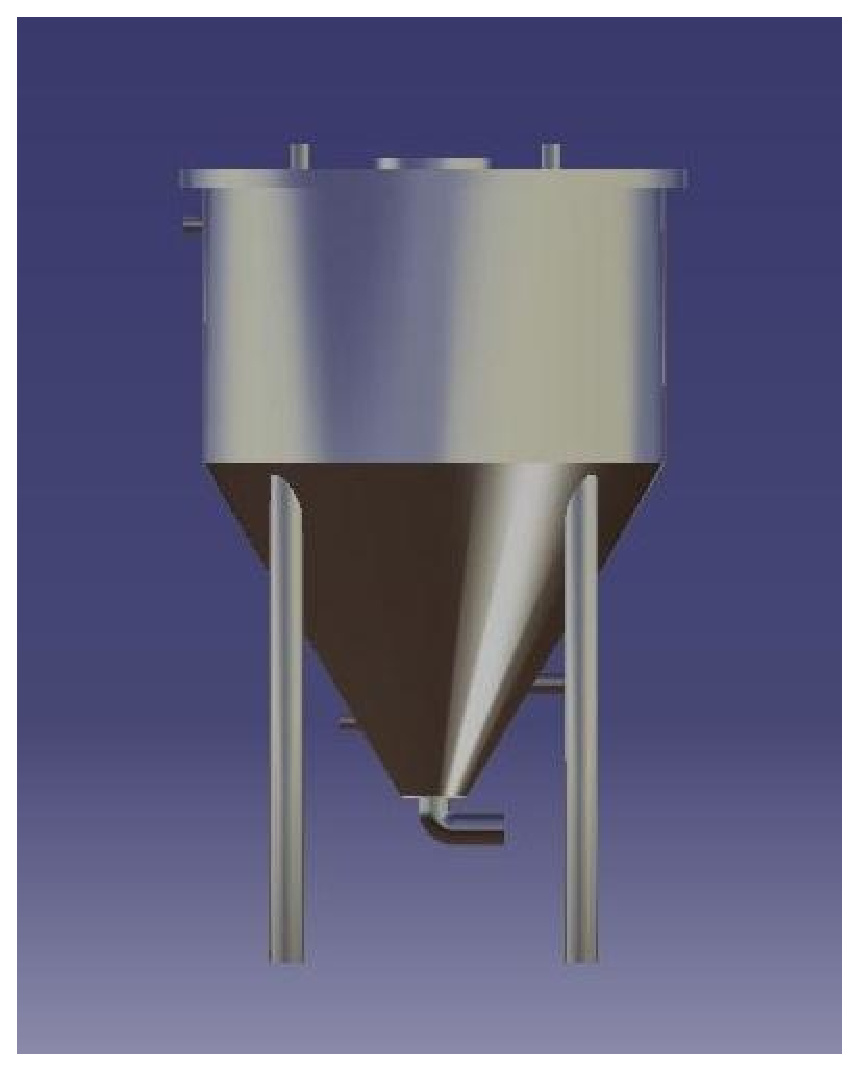
\includegraphics[keepaspectratio=true,scale=0.5]{figuras/catia1.eps}
	\caption{Biorreator modelado no CATIA - Posição 1}
	\label{catia1}
\end{figure}

\begin{figure}[h]
	\centering
	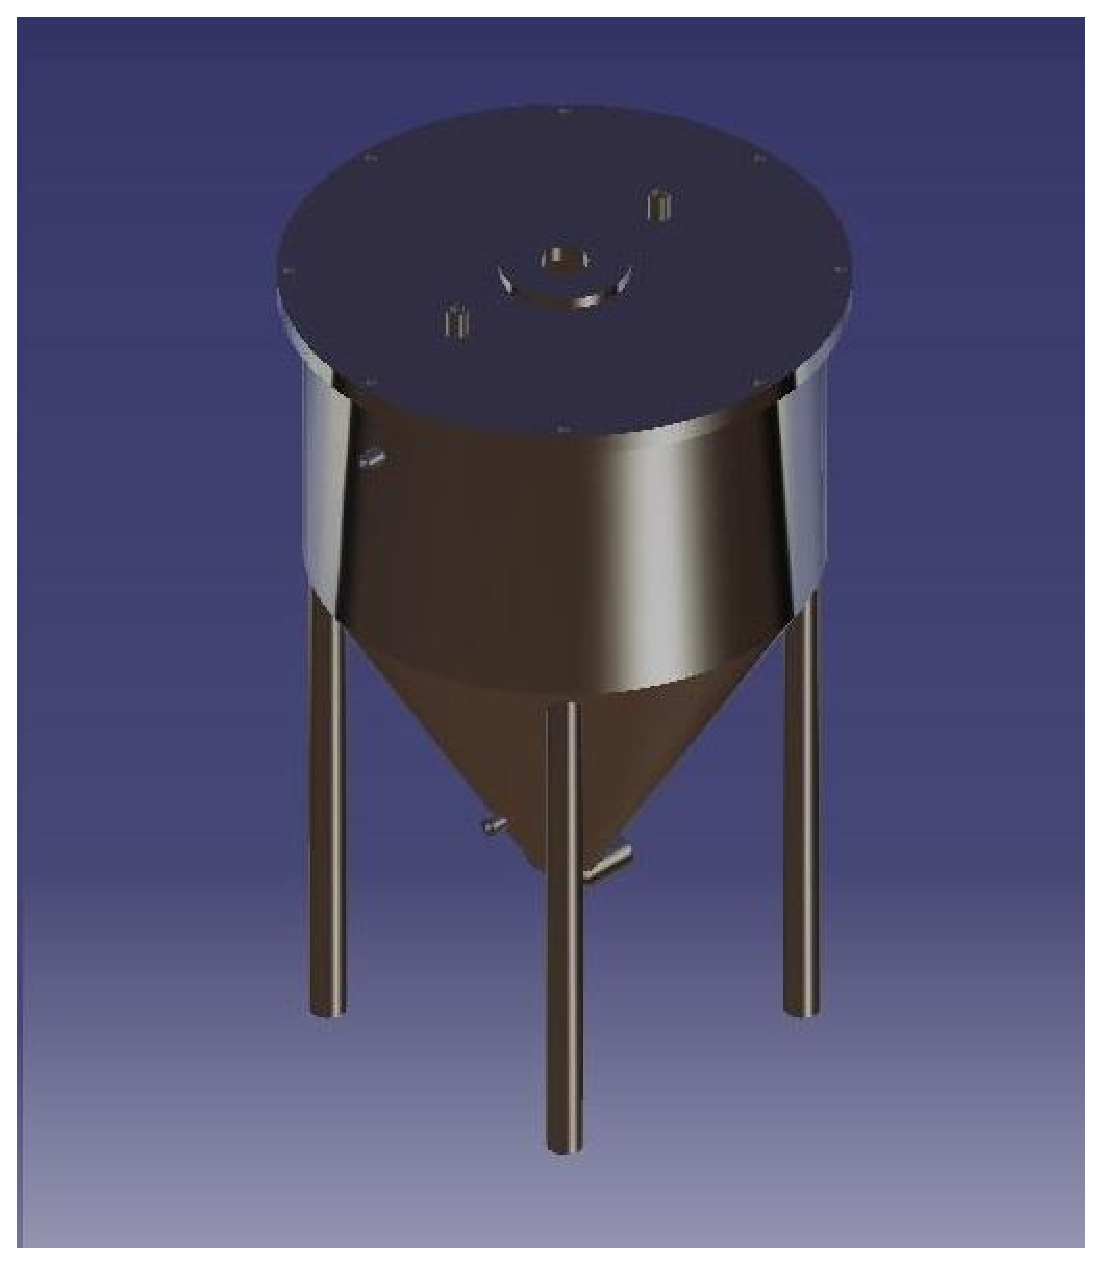
\includegraphics[keepaspectratio=true,scale=0.4]{figuras/catia2.eps}
	\caption{Biorreator modelado no CATIA - Posição 2}
	\label{catia2}
\end{figure}

A modelagem será feita com possíveis correções entre o ponto de controle 1 e 2, para então ser utilizado um software para simulação térmica do biorreator no  \textit{ANSYS}.

\subsubsection{Eixo}

Eixos são elementos que transmitem potência ou movimento. Um projeto de eixo visa atender a critérios de rigidez e deflexão, de resistência estática e à fadiga, além de uma análise de suas velocidades críticas. \cite{shigley2005projeto}

O critério de rigidez visa atender uma inclinação máxima que o eixo possa ter na região dos mancais. Essa inclinação máxima depende dos tipos de rolamentos empregado. Para atender os critérios de resistência existem cinco critérios de falha mais comuns e são eles: Langer, Sodeberg, Goodman, DE-Gerber e ASME-elíptico. A Figura 1 mostra as curvas desses quatro critérios em função das tensões estáticas (\( \sigma \)e) e alternadas (\( \sigma \)a) atuando no eixo. \cite{shigley2005projeto}

\begin{figure}[h]
	\centering
	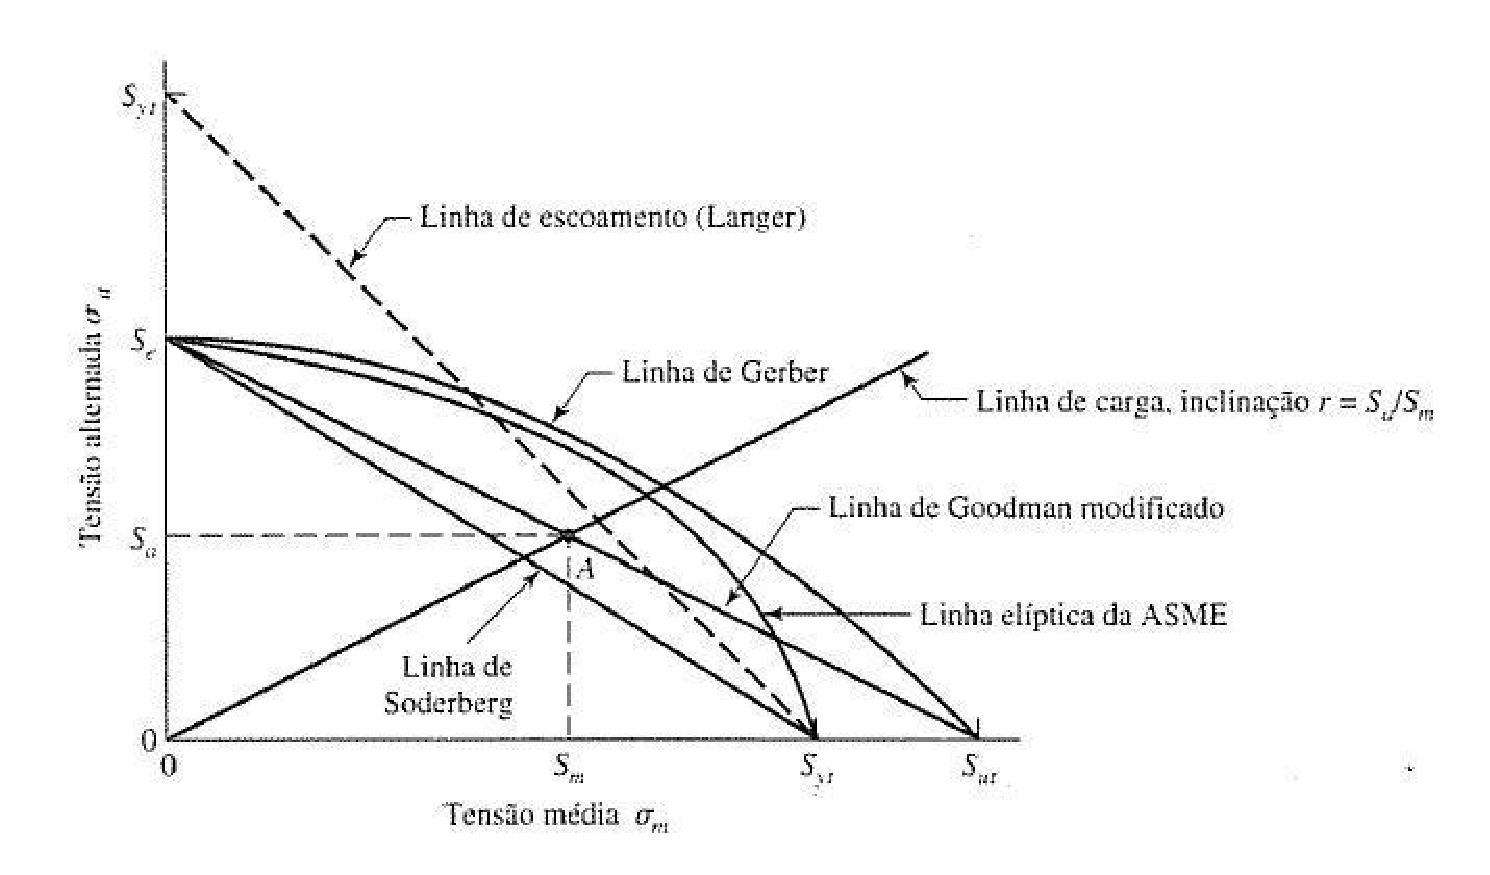
\includegraphics[keepaspectratio=true,scale=0.5]{figuras/eixo.eps}
	\caption{Critérios de falha em fadiga \cite{shigley2005projeto}.}
	\label{eixo}
\end{figure}

Dentre os materiais utilizados para fabricação de eixos, os aços são os materiais mais comuns. Isso se deve ao fato de possuírem um bom módulo de Young, o que se reflete diretamente numa melhora na questão de rigidez. Aços carbono SAE 1020-1050 são escolhas comum, porém quando as solicitações de resistência são muito elevadas alguns aços ligas podem ser utilizados como os SAE 3140, 4140-50, 4340. \cite{shigley2005projeto} Para aplicações em casos especiais, como o de atmosfera corrosiva, pode-se usar também os aços inoxidáveis.  \cite{norton2013projeto}.

O material de eixo a ser adotado para esse projeto é o aço inoxidável 304, por sua aplicabilidade em fermentações com risco de contaminação minimizados e também por conseguir atender os critérios de rigidez e resistência. O critério de resistência a fadiga a ser adotado é o critério de DE-Gerber por ser um critério menos conservador e acarretar em um eixo com um diâmetro menor.

\subsubsection{Rotor}

As pás do rotor serão construídas em material aço inox 304. As especificações para o projeto visa que o impelidor tenha aplicações em velocidade baixa a média, para misturas de baixa e média viscosidade. Os rotores que se inserem nesse perfil seriam rotores de pá cruzada, pá reta, pá pivotante dentre outras.

\begin{figure}[h]
	\centering
	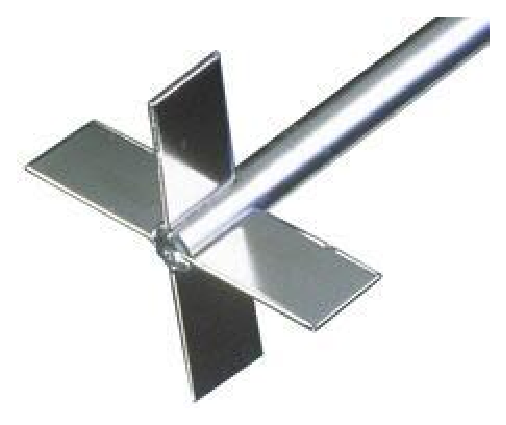
\includegraphics[keepaspectratio=true,scale=0.6]{figuras/pa.eps}
	\caption{Rotor de pá cruzada}
	\label{pa}
\end{figure}

O aço inoxidável 304 é classificado como aço inoxidável austenítico (aços não magnéticos), e possui características que enfatizam no uso para equipamentos na indústria química, depósitos de cerveja, tanques de fermentação, indústria farmacêutica dentre outras, sendo este aço com excelente aspecto para soldabilidade e estampabilidade \cite{kloeckner}.

\subsubsection{Flambagem}

As colunas que sustentam o biorreator sofrem com carregamentos axiais de compressão e podem, portanto, falhar por flambagem. A flambagem depende de diversos fatores, tais como o índice de esbeltez (Sr) das colunas e de suas respectivas condições de contorno. \cite{norton2013projeto}.

O valor do índice de esbeltez é responsável por caracterizar a coluna em coluna curta, a qual essa falhará por compressão, ou nas chamadas colunas longas, onde essa falhará por flambagem. O Sr depende do comprimento (l) da coluna e de propriedades de sua seção transversal, como a área (A) e o menor momento de inércia da seção transversal (I) . O índice de esbeltez é calculado a partir da equação 1. \cite{norton2013projeto}.

\[Sr = 1/\sqrt{\frac{I}{A}}\]

A Figura \ref{solda} mostra diversas condições de contorno e as curvas de deflexão da coluna para cada caso.

\begin{figure}[h]
 \centering
 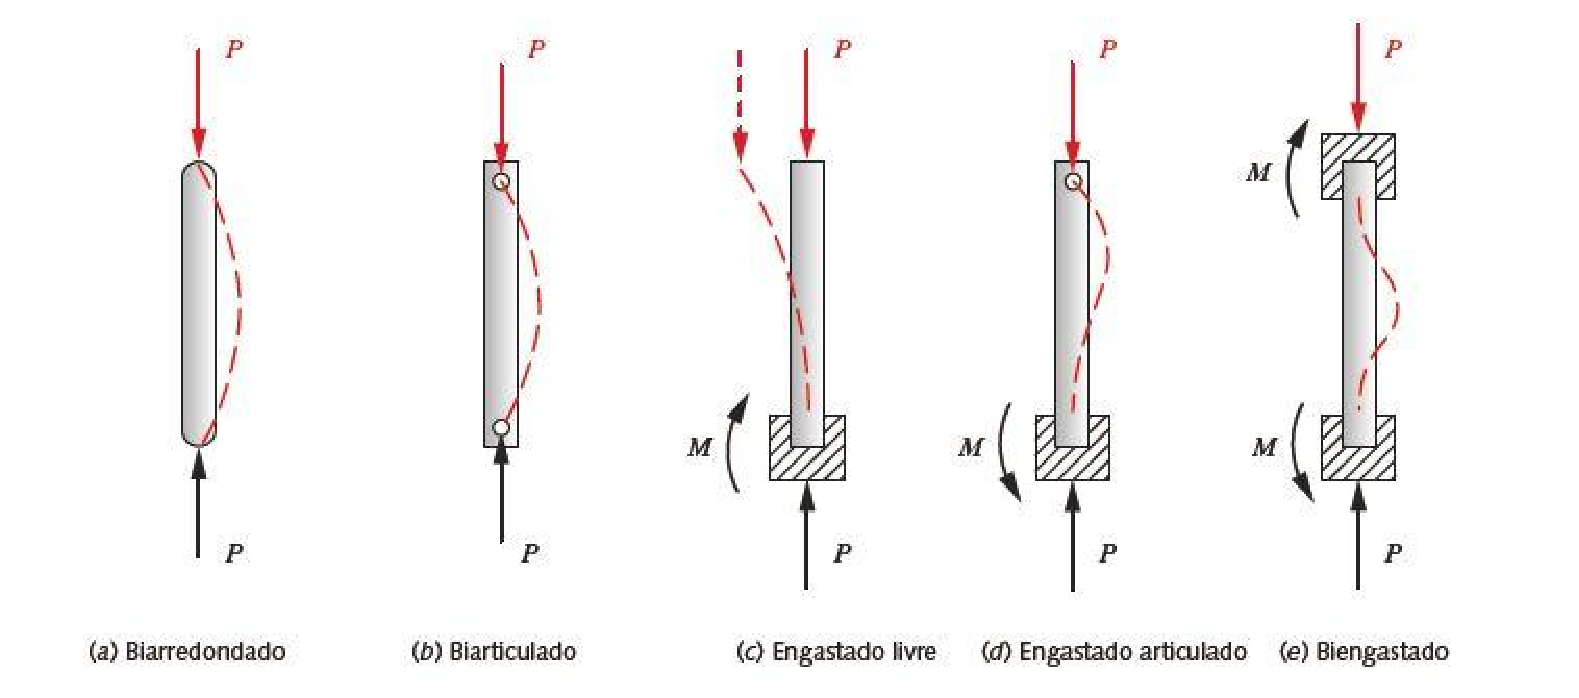
\includegraphics[keepaspectratio=true,scale=0.5]{figuras/solda.eps}
 \caption{Condições de contorno e curvas de deflexão.}
 \label{solda}
\end{figure}

\subsubsection{Dimensionamento do Motor do Impelidor}

O tipo de impelidor usado, seu diâmetro, a frequência do agitador o diâmetro do tanque, a altura da coluna líquida, a existência ou não de chicanas e sua largura, as características do líquido (densidade, viscosidade) são, segundo SCHMIDELL(2011) alguns exemplos das variáveis que afetam a potência que se transfere a um líquido submetido a agitação.

SCHMIDELL(2011) traz que uma estratégia  abordada para esse tipo de situação, consiste em lançar mão da análise dimensional, através da qual se busca juntar as variáveis em grupos dimensionais e, a seguir, obter as correlações entre esses adimensionais. Demonstrou-se que:

\[P = N^3  \times Di^5 \times \rho \times Np\]
\[NRe = (N \times Di^2 \times \rho)/\mu\]
\[Np = f(NRe)\]

Onde:
\begin{itemize}
	\item Np = Número de potência;
	\item NRe = Número de Reynolds;
	\item N = frequência do agitador (rps ou s-1);
	\item \(\rho\) = Densidade do líquido (kg/m3);
	\item P = Potência transmitida na agitação (W);
	\item Di = diâmetro do impelidor (m);
	\item \(\mu\) = Viscosidade do líquido (Kg/m \(\times\) s)
\end{itemize}

De acordo com o gráfico Np x NRe, figura \ref{reynolds}, determina-se o valor de o valor do número de potência:

\begin{figure}[H]
	\centering
  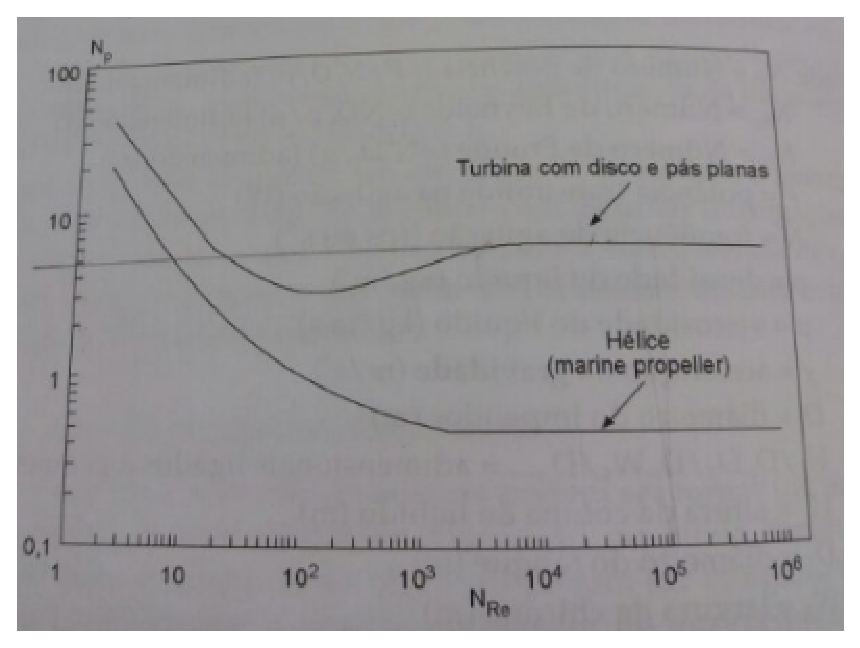
\includegraphics[keepaspectratio=true,scale=0.6]{figuras/reynolds.eps}
  \caption{  Número de potência \(\times\) Número de Reynolds. Fonte: SCHMIDELL,2011}
  \label{reynolds}
\end{figure}

Para a se obter a viscosidade e a densidade do líquido, que é a mistura de caldo de cana mais as leveduras, foram realizados ensaios no laboratório de química do Galpão. Os ensaios foram realizados com o líquido na temperatura de 31 ºC, pois é essa a temperatura durante a fermentação. O ensaio com o viscosímetro permitiu encontrar o valor da viscosidade cinemática (\(\upsilon\)) e por meio da pesagem de um volume determinado do líquido em uma balança de precisão foi encontrado o valor da densidade (\(\rho\)). Para a realização destes ensaios considerou-se  que para cada 1 litro de caldo de cana usa-se 10 g de levedura.

\begin{figure}[h]
	\centering
  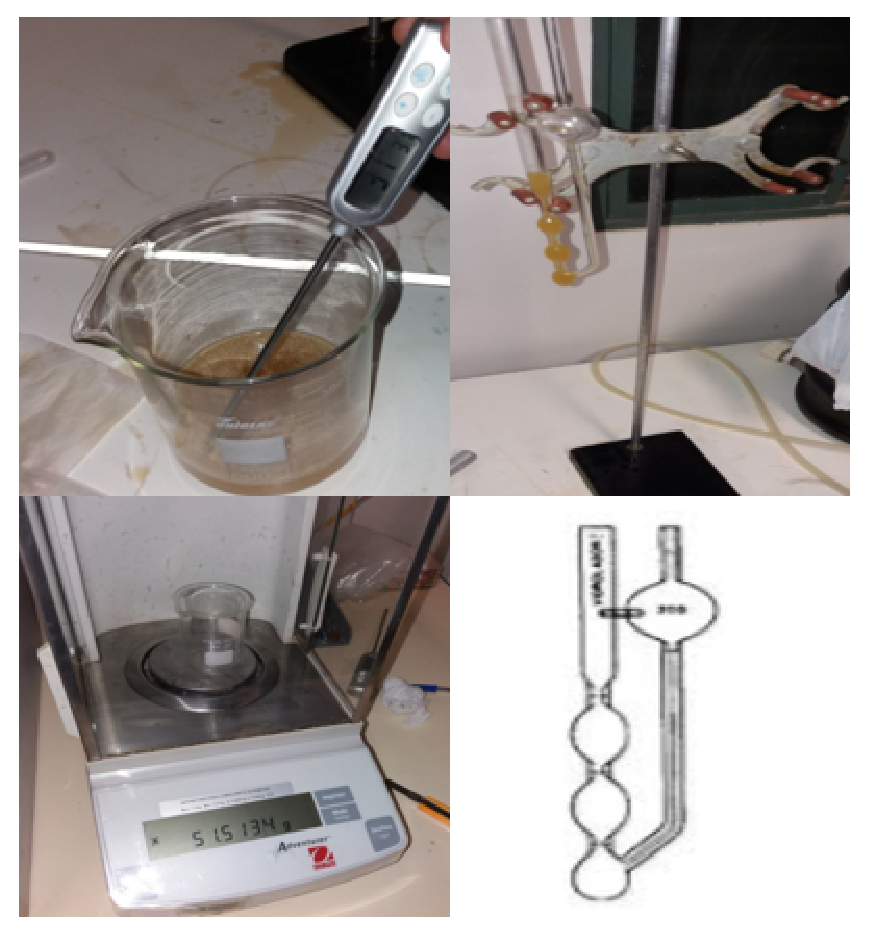
\includegraphics[keepaspectratio=true,scale=0.5]{figuras/equipamentos.eps}
  \caption{Equipamentos para medir viscosidade e densidade}
  \label{equipamentos}
\end{figure}

O valor encontrado para densidade foi 1065,51 kg/m3 e o valor da viscosidade cinemática foi 2,879 cts. A partir da relação:
\[\mu = \rho \times \upsilon\]

Encontrou-se o valor da viscosidade dinâmica (\(\mu\)) igual a 2,9397 cp.
Considerando que o impelidor é o modelo com pás planas, com diâmetro do impelidor igual a 155 mm, uma frequência de agitação de 150 Rpm que é a rotação usada em reatores de fermentação alcoólica (alguma referência), foi encontrada uma potência de aproximadamente 16 W.

\begin{figure}[H]
	\centering
  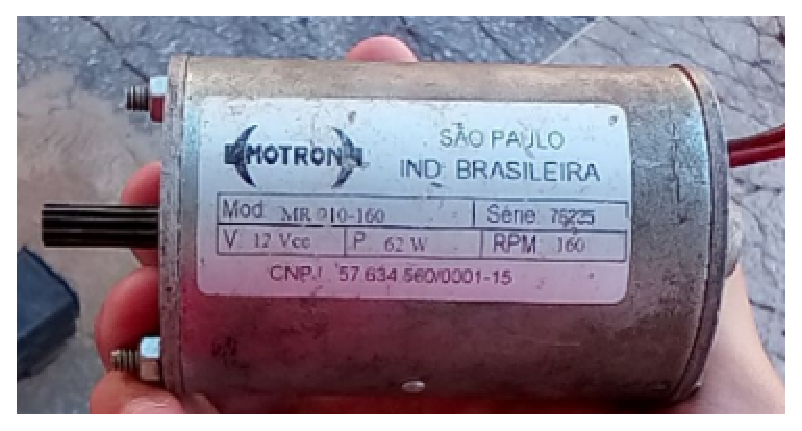
\includegraphics[keepaspectratio=true,scale=0.5]{figuras/motor.eps}
  \caption{Motor que será utilizado para agitação}
  \label{motor}
\end{figure}

\begin{figure}[H]
	\centering
  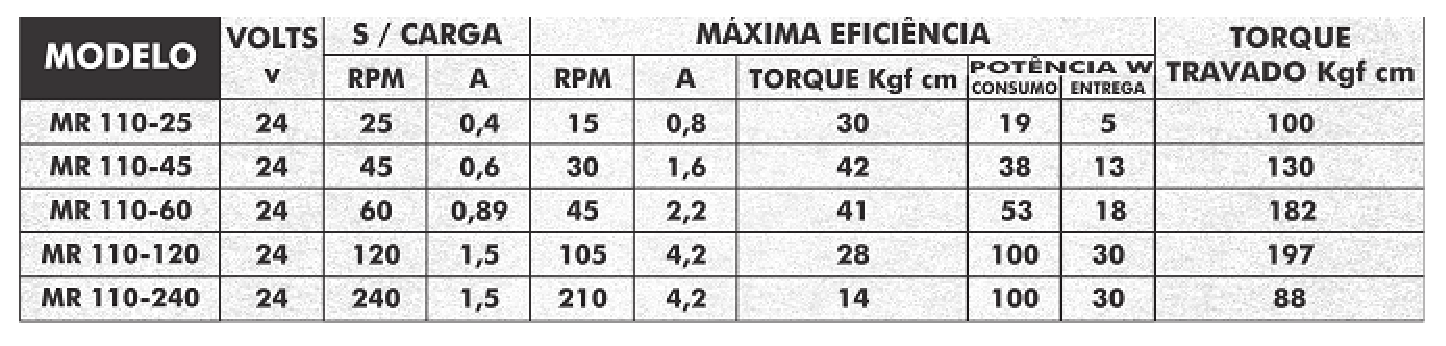
\includegraphics[keepaspectratio=true,scale=0.5]{figuras/data.eps}
  \caption{Datasheet do Motor que será utilizado para agitação}
  \label{data}
\end{figure}

\subsubsection{Soldagem}

Dentre os processos de soldagem mais difundidos na indústria, estão a soldagem a arco, soldagem a gás, soldagem por brasagem, soldagem por resistência e soldagem por laser. Para a soldagem aplicada no biorreator, devido a especificação do uso de aço inoxidável, será empregada a técnica de soldagem a arco. Este processo caracteriza-se pela participação do material base na fusão que constituirá a solda \cite{chiaverini1986tecnologia}.

O processo de soldagem que possibilita soldar a maioria dos metais e ligas, como, aços comuns, aços especiais (caso do aço inoxidável), alumínio, magnésio, cobre dentre outros é conhecido como processo de soldagem a arco com proteção de gás argônio, também chamado de TIG, pertinente ao uso de um eletrodo de tungstênio não consumível. O tungstênio possui a característica de suportar alta intensidade de corrente o que viabiliza o uso para obter grande quantidade de calor em uma área concentrada \cite{chiaverini1986tecnologia}.

\begin{figure}[h]
 \centering
 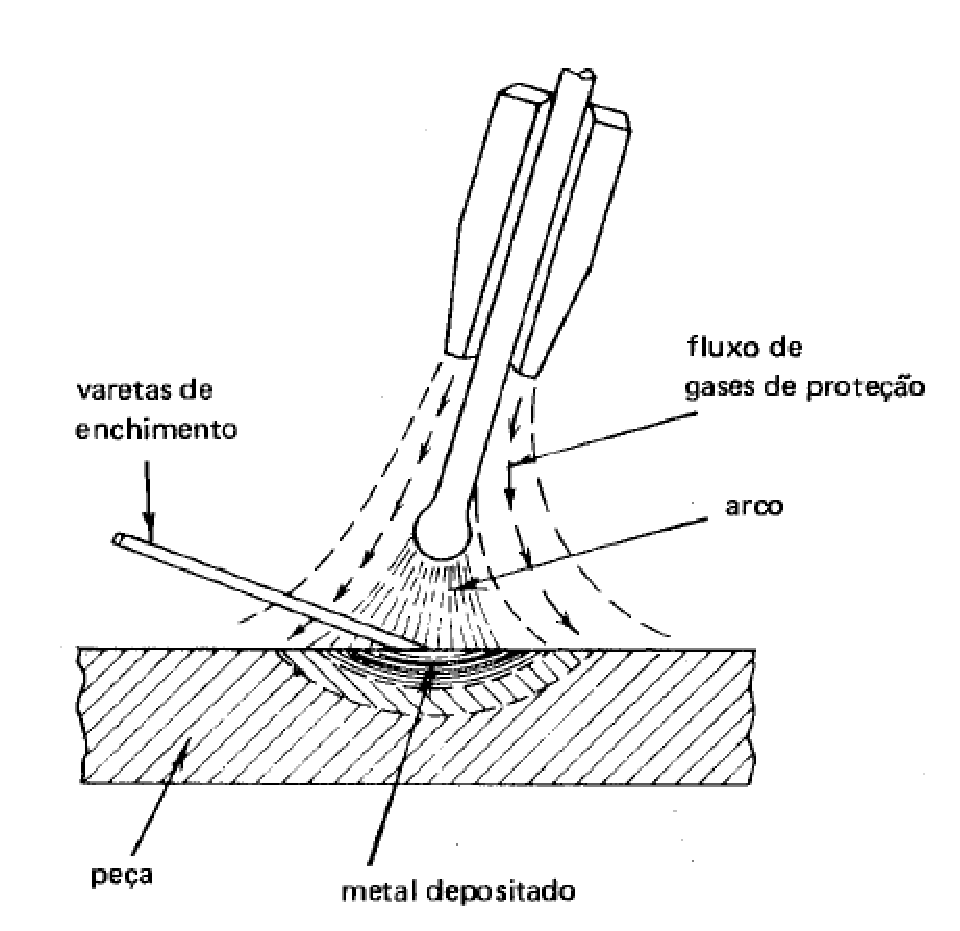
\includegraphics[keepaspectratio=true,scale=0.5]{figuras/contorno.eps}
 \caption{Soldagem por arco com proteção de gás argônio}
 \label{contorno}
\end{figure}

\subsection{Processos Termoquímicos}

A temperatura dentro do biorreator não possui uniformidade em todas as regiões, uma vez que o calor provocado pela fermentação não ocorre a uma taxa constante. Dessa forma, torna-se necessário o uso de múltiplos sensores de temperatura, para um monitoramento mais preciso \cite{silveira2009analise}. Uma das características do biorreator proposto é a variação da temperatura em uma faixa de 0 a 100ºC com controle automático PID no aquecimento. Os sistemas de resfriamento e aquecimento serão separados, uma vez que o resfriamento só ocorrerá ao final da reação com a finalidade de resfriar o mosto para etapas posteriores do processo, ou como medida de segurança para o caso de superaquecimento do biorreator.

\subsubsection{Sistema de resfriamento}

O ciclo de refrigeração é definido como uma região onde o fluido refrigerante circula, permutando em líquido e vapor de forma que viabilize a transferência de calor de um objeto onde ocorre a evaporação, processo que absorve calor, com baixa pressão e temperatura e a condensação, situação a qual rejeita calor, com alta pressão e temperatura. A temperatura dentro do cilindro do biorreator não possui uniformidade em todas as regiões, uma vez que o calor provocado pela fermentação não ocorre a uma taxa constante. Dessa forma, torna-se necessário o uso de múltiplos sensores de temperatura, para um monitoramento mais preciso \cite{silveira2009analise}.

Segundo \cite{mcketta1991heat} os tipos de sistemas de resfriamento estão em escala crescente a seguir

\textbf{Jaqueta Simples:} A jaqueta simples, ou camisa simples, possui de 2 a 3 polegadas de espaço anular na qual o fluido percorre lentamente. Ele é voltado para aplicações com baixa necessidade de transferência de calor.

\begin{figure}[h]
	\centering
	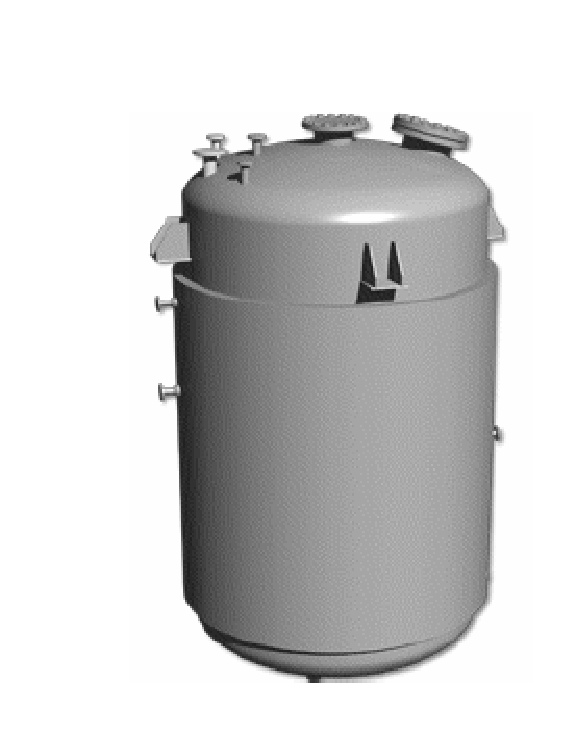
\includegraphics[keepaspectratio=true,scale=0.4]{figuras/jaqueta.eps}
	\caption{Jaqueta simples \cite{silveira2009analise} }
	\label{jaqueta}
\end{figure}

\textbf{Jaqueta com defletores em espiral:} A jaqueta com defletores consiste em um espiral longo de metal que direciona velocidades de fluido um pouco acima em relação as jaquetas simples.

\begin{figure}[h]
	\centering
	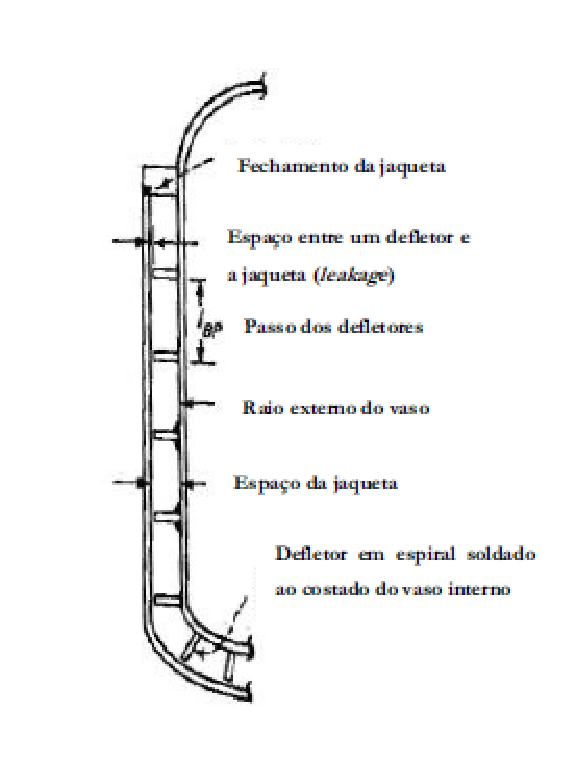
\includegraphics[keepaspectratio=true,scale=0.6]{figuras/jaqueta2.eps}
	\caption{Imagem em corte de jaqueta com defletores\cite{silveira2009analise}}
	\label{jaqueta2}
\end{figure}

\textbf{Jaqueta tipo dimple:} A jaqueta dimple possui a característica de não afetar a resistência sendo construído a partir de materiais mais leves.

\begin{figure}[h]
	\centering
	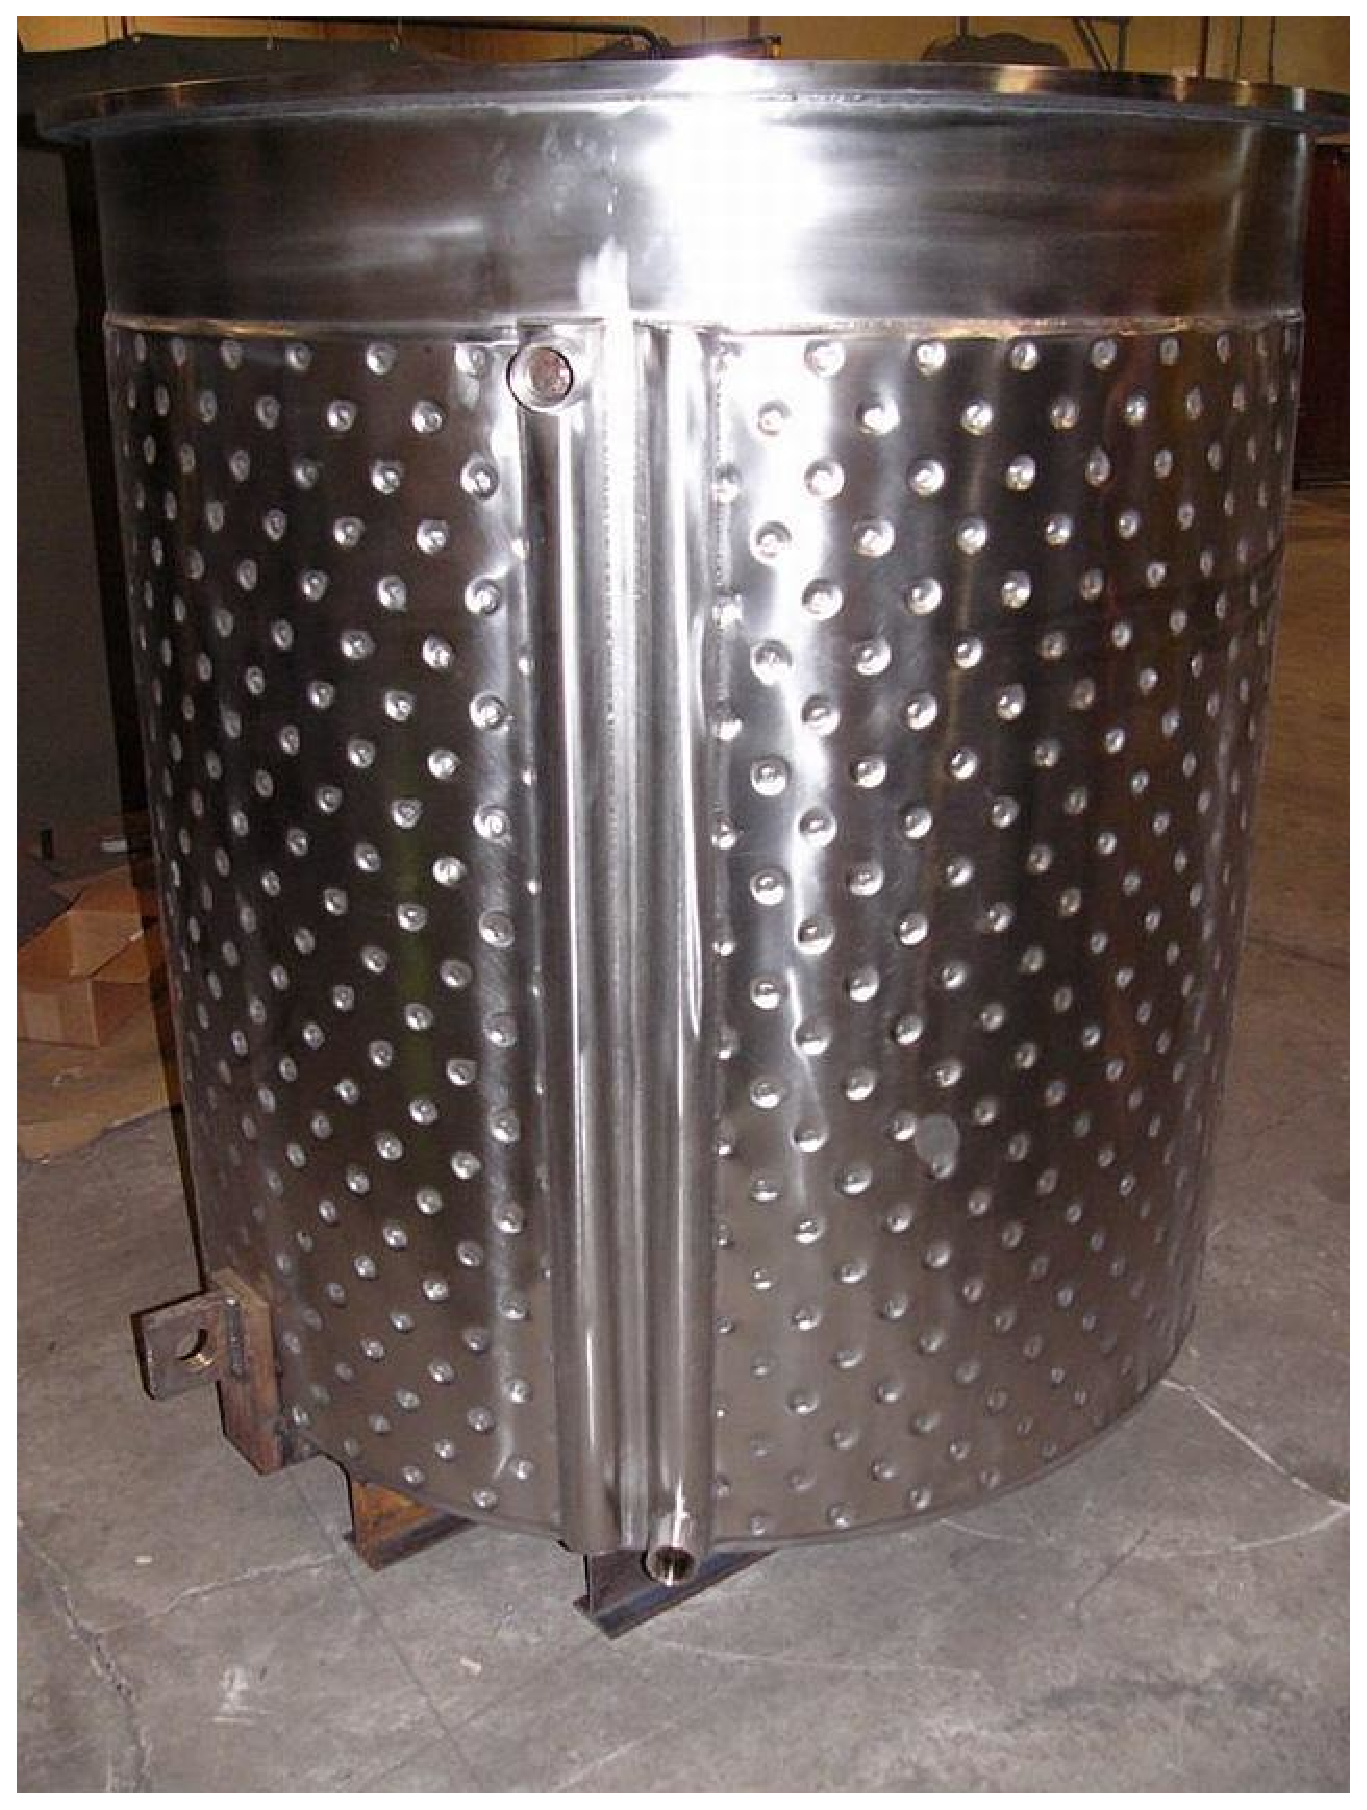
\includegraphics[keepaspectratio=true,scale=0.2]{figuras/jaqueta3.eps}
	\caption{Jaqueta Dimple. Fonte: Royal Welding - Site de Internet}
	\label{jaqueta3}
\end{figure}

\textbf{Jaqueta de serpentina meia-cana:} A jaqueta meia cana eleva a rigidez da estrutura, sendo os tubos soldados a parte externa do vaso.

\begin{figure}[h]
	\centering
	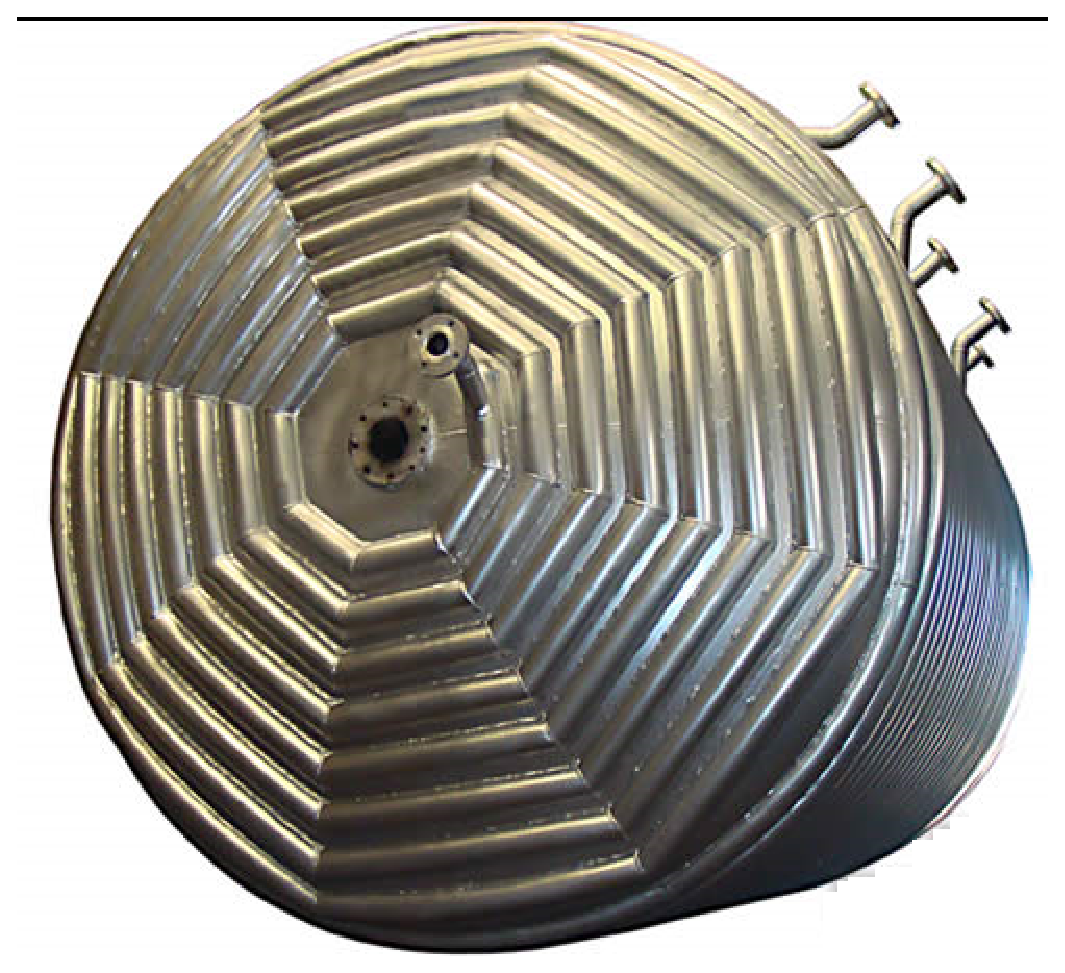
\includegraphics[keepaspectratio=true,scale=0.2]{figuras/jaqueta4.eps}
	\caption{Jaqueta meia-cana. Fonte: Metalúrgica Metalnox - Site de Internet}
	\label{jaqueta4}
\end{figure}

\textbf{Chapa integral ou jaqueta com serpentina tipo painel:} Esse tipo de serpentinas possuem a característica de transferir calor com controle e efetividade, podem ser utilizados fluidos em altas temperaturas, são fabricadas em materiais acessíveis, entretanto, esse tipo de sistema é mais caro do que aqueles que possuem serpentina interna \cite{mcketta1991heat}

\begin{figure}[h]
	\centering
	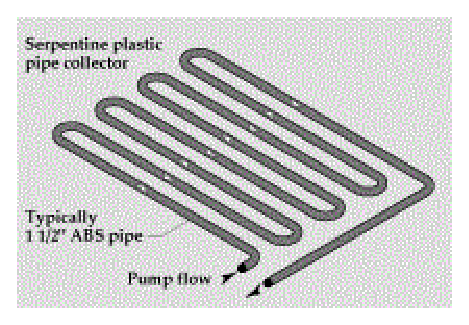
\includegraphics[keepaspectratio=true,scale=0.8]{figuras/serpentina.eps}
	\caption{Serpentina tipo painel. Fonte: Wikipedia - Site de Internet}
	\label{serpentina}
\end{figure}

Dos modelos de serpentina que serão estudados para ver qual se adequa melhor ao projeto, se tem 3 opções:

\begin{itemize}
  \item \textbf{Serpentina completamente dentro do reator:} Se escolhida essa opção o materialda serpentina será de aço inox, para evitar contaminação do mosto;
  \item \textbf{Serpentina parcialmente dentro do reator:} A serpentina passaria por pontos específicos do reator, para diminuir consideravelmente o acúmulo de mosto nos enrolamentos da estrutura;
  \item \textbf{Serpentina completamente fora do reator, em volta da parte externa:} Nesse caso teria a necessidade de adicionar um material isolante em volta da serpentina para que não houvesse interferência do ambiente na troca de calor;
\end{itemize}

Além dos sistemas citados, outra opção interessante é o uso de pastilhas termoelétricas do tipo \textit{Peltier}. Elas são um cooler termoelétrico com a capacidade de aquecer e resfriar objetos em minutos com a simples alimentação dos seus terminais. Ou seja, seu princípio de funcionamento se consiste basicamente na passagem de corrente elétrica contínua entre dois metais diferentes e com isso, aplica-se uma voltagem entre os pólos, que por consequência, um diferencial de temperatura entre as faces opostas das placas, é criado. Importante ressaltar que apesar da pastilha ter a capacidade de aquecimento, nesse projeto ela será usada apenas para resfriar, uma vez que o sistema de aquecimento é separado e controlado de forma PID.

Após ligar a pastilha \textit{Peltier} um lado irá aquecer rapidamente, enquanto o outro esfriará, contudo para que não entre em equilíbrio e comprometa a pastilha é necessário um dissipador de calor do lado quente. Essa partilha será ligada em uma fonte de 12V. A Figura \ref{pastilhas} mostra o funcionamento simplificado de como essas pastilhas funcionam, com relação a transferência de calor.

\begin{figure}[h]
	\centering
	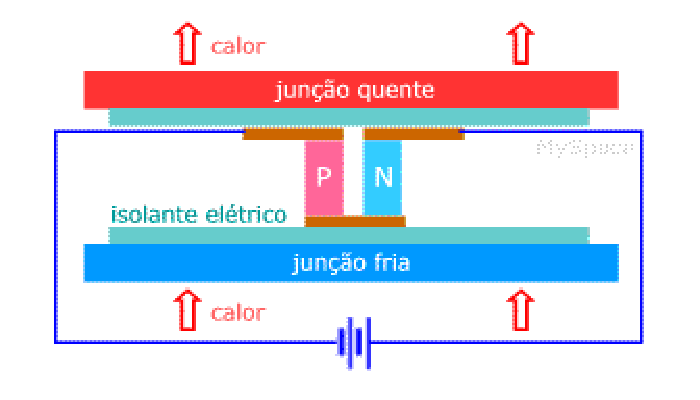
\includegraphics[keepaspectratio=true,scale=0.6]{figuras/pastilhas.eps}
	\caption{Funcionamento das pastilhas termoelétricas}
	\label{pastilhas}
\end{figure}

A figura a seguir mostra um sistema esquemático do sistema termoelétrico do efeito \textit{Peltier}, já acoplado com os respectivos dissipadores e ventiladores, componentes estes, essenciais para o adequado funcionamento do sistema.

\begin{figure}[h]
	\centering
	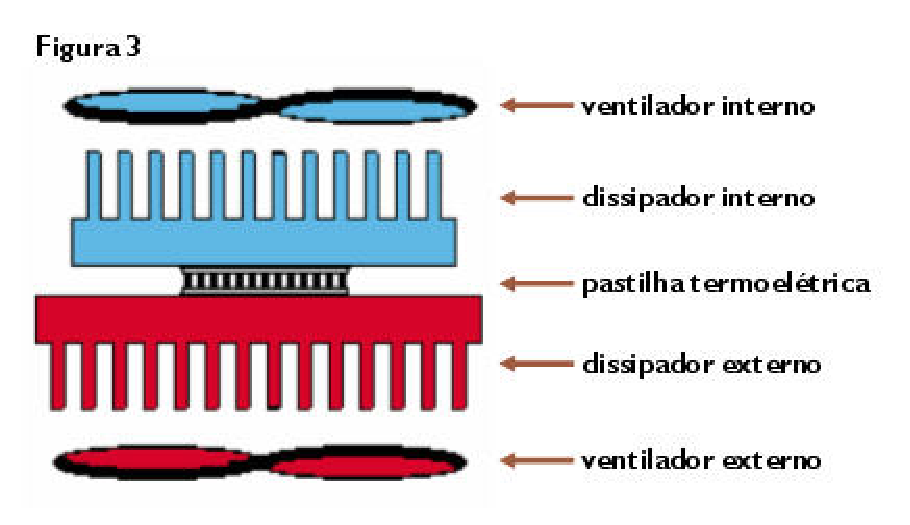
\includegraphics[keepaspectratio=true,scale=0.6]{figuras/peltier.eps}
	\caption{Esquema do efeito Peltier}
	\label{peltier}
\end{figure}

Um modelo bastante conhecido é a Pastilha Termoelétrica Peltier EC1-12706 Cooler.

\begin{figure}[h]
	\centering
	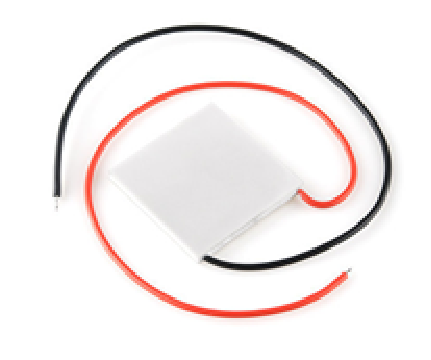
\includegraphics[keepaspectratio=true,scale=0.6]{figuras/cooler.eps}
	\caption{Pastilha Termoelétrica Peltier EC1-12706 Cooler}
	\label{cooler}
\end{figure}

Suas especificações são citadas abaixo:
\begin{itemize}
  \item Faixa de Temperatura: -30 a 70 Celsius;
  \item Tensão de operação: 0 -15,2 VDC;
  \item Corrente de operação: 0 - 6 A;
  \item Potência máxima: 60W;
  \item Dimensões: 40 x 40 mm
  \item Preço médio: R\$ 22,90
\end{itemize}

Em relação ao conjunto célula \textit{Peltier}, dissipador de calor e ventilador (ventoinha) encontrou-se duas possibilidades. A primeira seria comprar um radiador frigorífico (conjunto de resfriamento com os três respectivos elementos já montados), figura \ref{radiador}.

\begin{figure}[h]
	\centering
	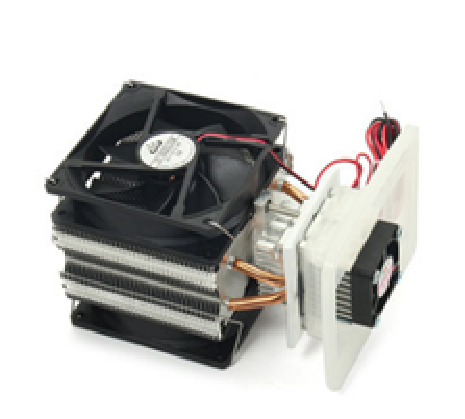
\includegraphics[keepaspectratio=true,scale=0.5]{figuras/radiador.eps}
	\caption{Radiador para refrigeração}
	\label{radiador}
\end{figure}

Em seguida ligá-lo a uma fonte de alimentação, figura \ref{radiador2}. O preço encontrado para um radiador, modelo Geekcreit® 12V 6A DIY foi em média de R\$ 68,00.

\begin{figure}[h]
	\centering
	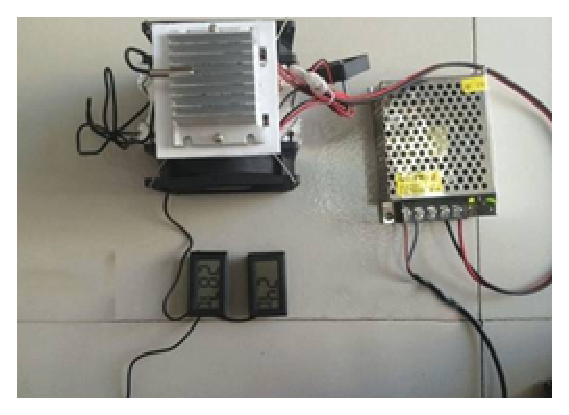
\includegraphics[keepaspectratio=true,scale=0.6]{figuras/radiador2.eps}
	\caption{Radiador conectado à fonte de 12 V}
	\label{radiador2}
\end{figure}

A segunda seria comprar os elementos separados e uni-los. Ao se realizar um estudo mais detalhado de custos a alternativa mais econômica será escolhida.

Baseando-se no uso de células \textit{Peltier} , a água em um reservatório será resfriada e esse líquido sob baixa temperatura será bombeado para que possa percorrer a serpentina que vai estar acompanhada do reator. Um modelo simplificado deste sistema é mostrado na figura \ref{resfriamento}:

\begin{figure}[h]
	\centering
	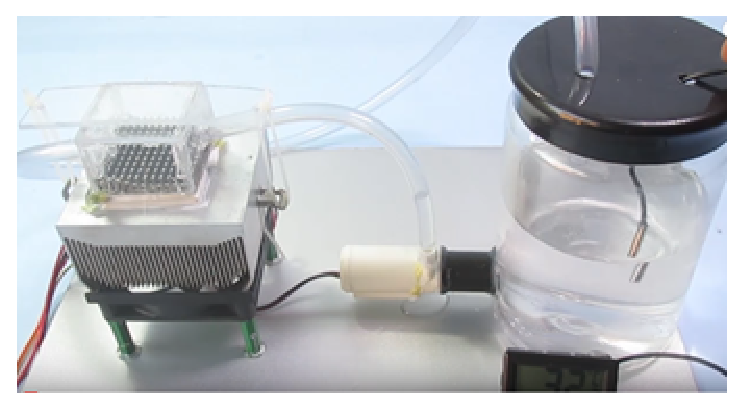
\includegraphics[keepaspectratio=true,scale=0.5]{figuras/resfriamento.eps}
	\caption{Modelo básico do sistema de resfriamento}
	\label{resfriamento}
\end{figure}

\subsubsection{Sistema de aquecimento}

Foram estudados alguns sistemas de aquecimento para o presente Biorreator e várias técnicas foram encontradas, como a  cinta térmica de silicone, que fica na parte externa à estrutura e proporciona uma transferência de calor para o fluido contido no reator, de acordo com a faixa de temperatura que se deseja, controlada através de um termostato, que oscilam de 0º a 90º ou 40º a 210º.

\begin{figure}[h]
	\centering
	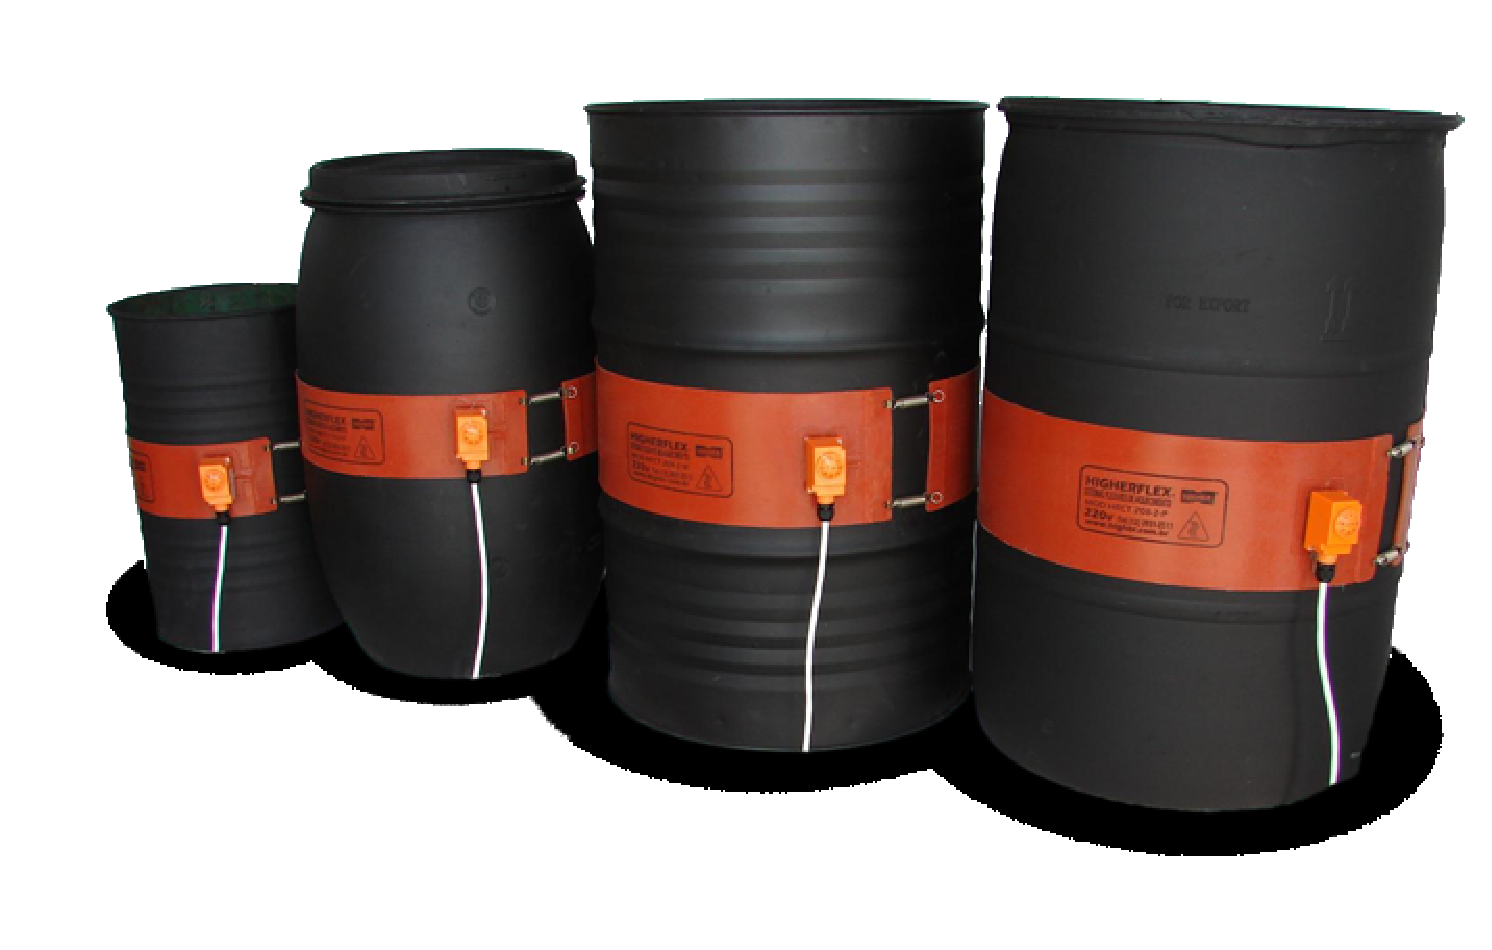
\includegraphics[keepaspectratio=true,scale=0.3]{figuras/cinta.eps}
	\caption{Modelos de cintas térmicas de silicone para diversos tamanhos de tambores}
	\label{cinta}
\end{figure}

A cinta elétrica de silicone fornece aquecimento rápido e eficaz, tendo vida útil longa e possui uma fácil aplicação, o que facilitaria o seu uso quando for necessário, já que o aquecimento seria utilizado em algumas situações específicas, pois trata-se de um biorreator genérico, onde envolverá diferentes tipos de fermentação. Este tipo de cinta é projetada para espalhar de forma eficiente o calor sobre a face do biorreator e o controle preciso de temperatura é obtido através do termostato que proporciona um aquecimento uniforme, como ilustra a Figura a seguir:

\begin{figure}[h]
	\centering
	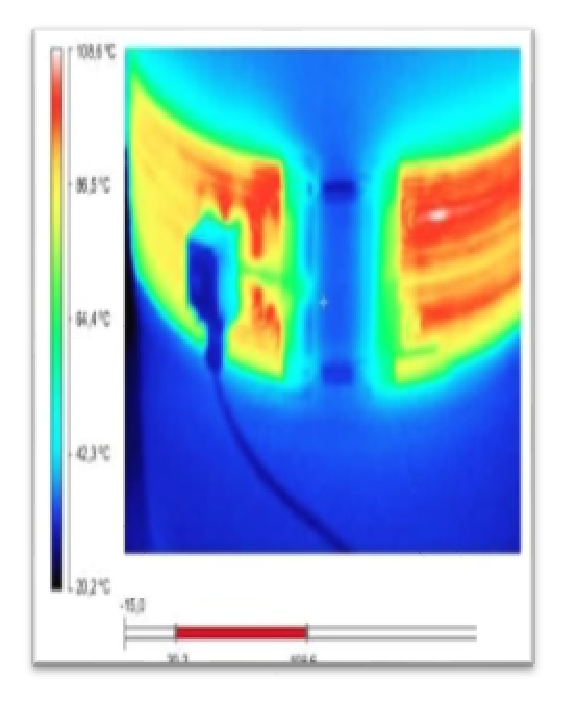
\includegraphics[keepaspectratio=true,scale=0.4]{figuras/cinta2.eps}
	\caption{Simulação de transferência de calor da cinta.
Fonte: higher.com.br}
	\label{cinta2}
\end{figure}

Outra forma que foi encontrada para o sistema de aquecimento foi a utilização de resistência elétrica para aquecer o fluido presente no reator. Essas resistências convertem energia elétrica em calor por meio do processo de dissipação de calor pelo aquecimento Joule, onde uma corrente elétrica aquece um condutor por meio da resistência inerente a ele. Um dos pontos positivos em sua utilização é que a resistência elétrica pode ser submetida a severas condições de trabalho sem prejudicar seu próprio funcionamento.

Atualmente, as resistências elétricas são constituídas de ligas de níquel e crômio que suportam temperatura de até 1000 ºC, são resistentes e também inoxidáveis.

Nas aplicações industriais, este tipo de sistema de aquecimento é mais utilizado devido a sua arquitetura de posicionamento. Em biorreatores, a resistência é utilizada pois sua instalação é feita dentro do próprio reator de forma que toda ela esteja em contato com o fluido que será aquecido, desta forma se tornou mais viável o estudo deste sistema de aquecimento, ilustrado na Figura \ref{resistencia}.

\begin{figure}[h]
	\centering
	\includegraphics[keepaspectratio=true,scale=0.2]{figuras/resistencia.eps}
	\caption{Resistência para aquecimento}
	\label{resistencia}
\end{figure}

O funcionamento do sistema de aquecimento consistirá na alimentação da resistência com corrente provinda do sistema de alimentação, para que a potência seja estabelecida e então o aquecimento aconteça. Para o controle da temperatura do fluido, o sistema de aquecimento trabalhará em conjunto com controle eletrônico na forma de controlador PID \textit{(Proporcional-Integral-Derivativo)}, que funciona como um controlador de temperatura.

 O controlador PID é integrado com um sensor de temperatura, desta forma ele calcula uma resposta de saída para a resistência, realizando assim o rampeamento da temperatura e por consequência seu controle. Os controladores PID servem para que não aconteça variação de temperatura e que a resistência mantenha o fluido em um temperatura constante. A Figura \ref{pid} ilustra um dos tipos de controladores PID.

 \begin{figure}[h]
 	\centering
 	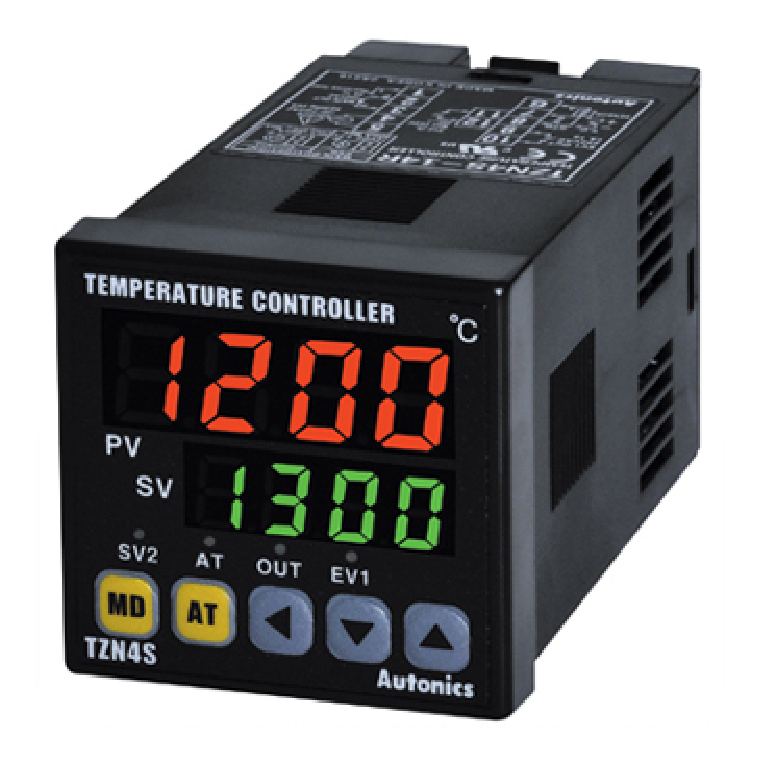
\includegraphics[keepaspectratio=true,scale=0.3]{figuras/pid.eps}
 	\caption{PID para controle de temperatura. Fonte: Ballast Conectors}
 	\label{pid}
 \end{figure}

\subsubsection{Sistema de Armazenamento de CO2}

A partir do cenário mundial, quanto a questões ambientais, o lançamento de gases poluentes no meio ambiente tem causado inúmeros prejuízos aos seres humanos. Com isso, protocolos e acordos ambientais foram criados, no decorrer dos anos, para que essas emissões fossem feitas de forma menos intensa. Devido a isto, a captura de CO2, advindos da fermentação de biorreatores, se torna extremamente importante para o meio ambiente.

O sistema de armazenamento de CO2 deste presente projeto será feito através de um outro sistema, acoplado ao biorreator, na qual o seu princípio de se consistirá na produção de microalgas em meio aquoso, através da fotossíntese. O seu funcionamento será similar ao de um aquário, onde microalgas serão colocadas na água e uma bomba (bomba de aquário) será responsável por fazer a oxigenação da mesma. Todo esse processo deverá ser feito na presença de luz, para assim ocorrer a fotossíntese.

A forma de captura deste gás gera ainda mais valores agregados a este projeto, pois as microalgas produzirão energia em forma de biomassa, viabilizando assim a produção de biocombustíveis.

\begin{figure}[h]
 \centering
 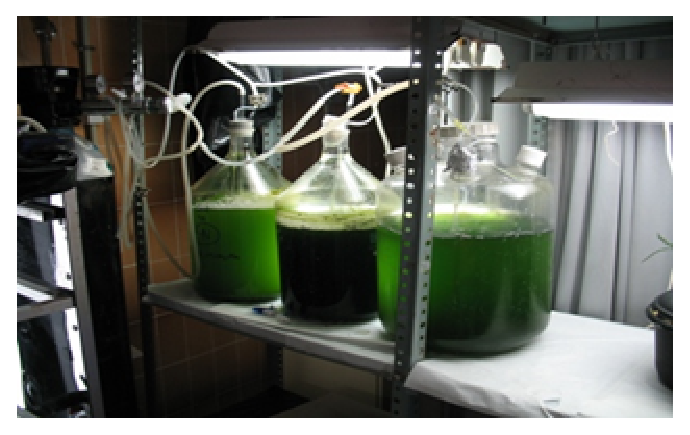
\includegraphics[keepaspectratio=true,scale=0.5]{figuras/algas.eps}
 \caption{Produção de microalgas. Fonte: dicasverdes.com}
 \label{algas}
\end{figure}

O sistema que será utilizado, acoplado ao biorreator, será similar ao mostrado na Figura \ref{algas}.

\subsubsection{Alimentação da Bancada}

A alimentação da bancada se consistirá em um cabo de energia com conexão tripolar (com fio terra) seguindo a padronização da Comissão Eletrotécnica Internacional – IEC. Constituída com uma potência de 220 V, o equivalente a 1200 W, em pleno funcionamento. Acredita-se que com todos os sensores e equipamentos que serão utilizados serão compatíveis com a alimentação informada, onde todos eles estarão interligados a este cabo de energia e a um sistema de software, que permitirá ou não o seu acionamento, de acordo com a necessidade de aplicação.

\subsection{Arquitetura}

\subsubsection{Comunicação entre os módulos}

A arquitetura de comunicação do sistema foi determinada pela disposição de módulos, sendo que para cada um existe a separação de suas responsabilidades, de forma que cada um destes cumpra uma única tarefa dentro do sistema para que exista uma melhor forma de controle e manutenção. Assim tanto a identificação de problemas no decorrer do desenvolvimento e de futuras atualizações como o trabalho paralelizado são possibilitados pela natureza de que cada um destes módulos se comporta como um serviço para o sistema como um todo.

O sistema irá possuir ao todo 6 módulos e os mesmos estão separados em 3 grupos de acordo com suas principais responsabilidades: controle, comunicação e interface. Os sensores e atuadores são os módulos presentes na área de controle, por serem responsáveis por controlar e atuar sobre os índices do sistema que serão captados. Enquanto os conversores, \textit{Raspberry} e a \textit{API} serão os módulos responsáveis pelo tratamento e comunicação de dados com o aplicativo que é a camada responsável pela apresentação e recepção de valores com o usuário final.

Os módulos serão desenvolvidos com as seguintes tecnologias:
\begin{itemize}
  \item Para comunicação e tratamento de dados vindo dos sensores através de uma interface com arduino será utilizada bibliotecas em C.
  \item Para comunicação e tratamento de dados vindo dos conversores AD/DA serão utilizadas bibliotecas em Python.
  \item Para construção da API será usado um framework javascript NodeJS e será hospedado no servidor do Heroku.
  \item O aplicativo será desenvolvido através de um framework javascript de cross-platform, React Native.
\end{itemize}

\begin{figure}[h]
 \centering
 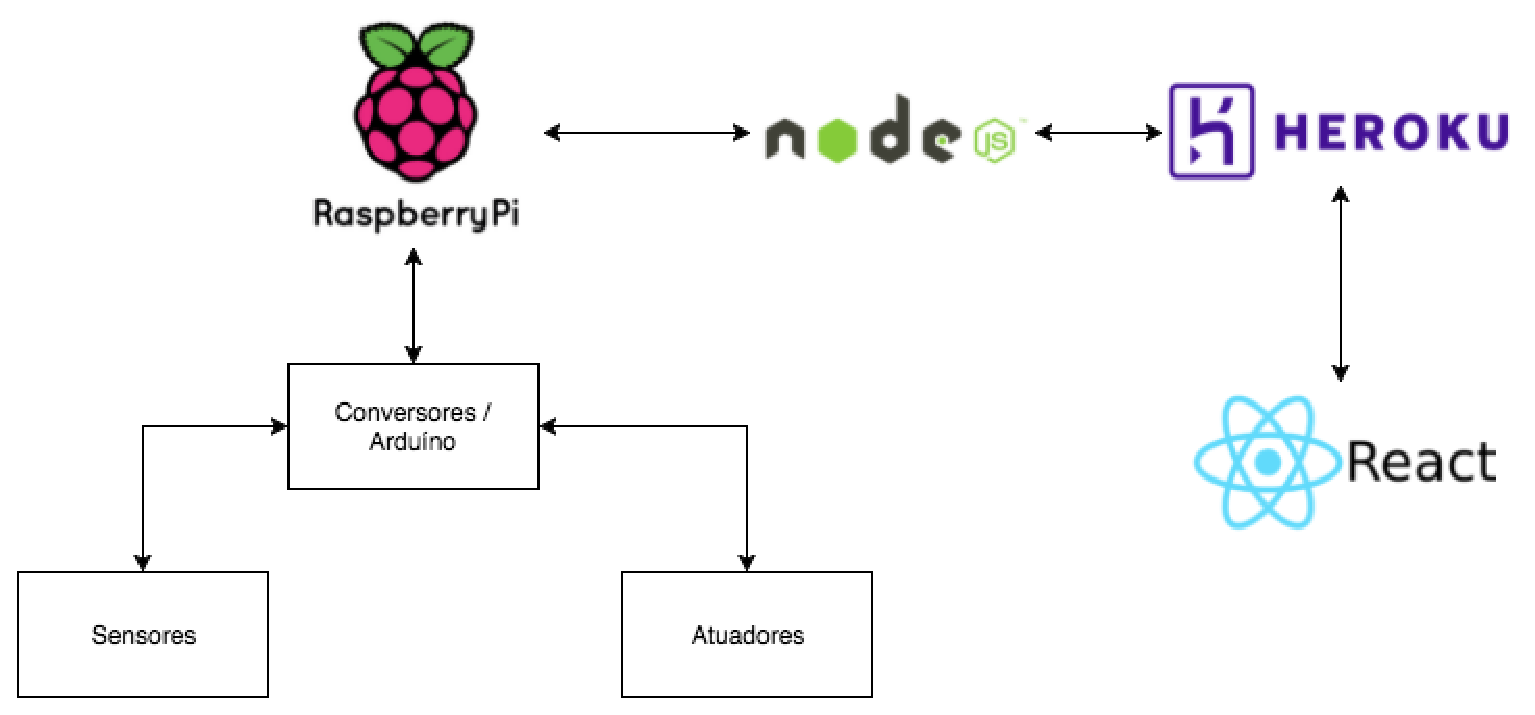
\includegraphics[keepaspectratio=true,scale=0.5]{figuras/arquitetura.eps}
 \caption{Arquitetura de monitoramento e controle}
 \label{arquitetura}
\end{figure}

\subsubsection{Especificação de Tecnologia de Software}

O sistema integrado de software terá como arquitetura duas camadas de comunicação, onde uma destas será o servidor responsável pelo tratamento e disponibilização dos dados vindos do sistema de sensores e a outra será a aplicação de interface com o usuário, onde serão apresentados gráficos e também recebidos inputs necessários para o sistema.

Para o servidor será utilizado um mecanismo de execução em Javascript, o NodeJS, que será responsável pelo serviço de \textit{REST}, que é uma abstração da arquitetura da \textit{World Wide Web} através de protocolos de comunicação \textit{HTTP} sendo aplicado à um web service fornecendo uma API para acesso do sistema de interface com o usuário. Como notação para transferência de dados será utilizado objetos \textit{JSON} para enviar as estruturas para o sistema de interface.

O sistema de interface com usuários será focado para uso mobile então será utilizado o \textit{framework} \textit{ReactNavite}, este é um \textit{cross-platform} em \textit{Javascript} que será responsável por gerar aplicativos para plataformas \textit{Android e iOS}. O aplicativo terá como função comunicar com a \textit{API} para recepção de dados que serão mostrados em relatórios ou para enviar dados que serão responsáveis por emitir sinais junto aos atuadores.

\section{Modelagem do Biorreator}

\subsection{Sistema de Aquecimento}

Um dos requisitos do projeto é que a temperatura varie de (0 a 100) ºC, com uso de uma resistência elétrica para aquecimento controlada por um controlador PID. Entretanto, segundo a avaliação realizada por De Sousa e Monteiro (2011) sobre perfil de reações de fermentação, a temperatura ideal para a operação das leveduras é de (25 a 30)ºC, sendo que temperaturas superiores ocasionam o enfraquecimento delas e favorece o surgimento de outros microorganismos inibidores de álcool, além de aumentar a perda de etanol por evaporação. Foi apontado ainda que temperaturas inferiores reduzem a atividade do fermento, diminuindo o rendimento do produto. Dessa forma,  foi modelado um sistema que varie de (25 a 40) ºC.

O sistema de aquecimento é composto basicamente da resistência elétrica e do controlador PID, que acompanha um termostato e um relé de estado sólido.

\begin{enumerate}
	\item Resistência Elétrica \\
	Uma vez que o biorreator é de uso genérico, ou seja, servirá para fermentar diversos tipos de mosto, não é possível definir a massa específica e densidade, já que tais parâmetros irão variar de acordo com o que será fermentado. Dessa forma, para os cálculos do dimensionamento da resistência será considerada uma densidade fixa que equivale à 18 ºBrix, valor mais propício para que a fermentação ocorra.

	Das especificações do reator se tem:
	\begin{itemize}
		\item Volume útil: 15 L
		\item Variação de temperatura: 15ºC
		\item 18º Brix \(\sim\) 1.075,07 \(kg.m^{-3}\)
	\end{itemize}

A partir da equação 1 é possível calcular a massa do mosto:

\[\rho = \frac{m}{v}\]

Onde:

\begin{itemize}
	\item \(\rho\): densidade
	\item m: massa
	\item v: volume
\end{itemize}

\[m = 1.075,07 Kg.m^{-3} 0,015 m^3\]

\[m = 16, 13 Kg\]

A equação 2 representa o cálculo da transferência de calor, em que uma de suas variáveis é o calor específico do mosto. Nesse caso será considerado o da cana de açúcar, que é o mosto padrão em reações de fermentação. A temperatura inicial será considerada ambiente 25ºC.

\[Q = m c \triangle T\]

Onde:

\begin{itemize}
	\item Q: Quantidade de calor
	\item m: massa [g]
	\item c: calor específico [J/Kg ºC]
	\item T: variação de temperatura
\end{itemize}


\[Q = 16,13 Kg \times 3,1J.Kg^{-1}K^{-1} \times (40 - 25)ºC\]
\[Q= 750 W\]

Assim, será necessário uma potência de 750 W. Comercialmente, não são produzidas resistências com tal potência, de forma que foi adquirido uma potência de 1000W (Figura \ref{resistencia}. Entretanto, como ela será controlada por PID, não haverá problemas da potência dela ser maior do que a dimensionada.

\begin{figure}[h]
 \centering
 \includegraphics[keepaspectratio=true,scale=0.2]{figuras/resistencia.eps}
 \caption{Resistência}
 \label{resistencia}
\end{figure}

Esse formato de resistência foi escolhido para aumentar a área de contato com o fluido. As especificações dela são dadas a seguir:

\begin{table}[h]
\centering
\caption{Especificações resistência}
\label{esp-rest}
\begin{tabular}{|l|c|}
\hline
Potência    & 1000W   \\ \hline
Bitola      & 3/8     \\ \hline
Comprimento & 25,5 cm \\ \hline
\end{tabular}
\end{table}

\item Controlador PID \\
A forma de controle PID consiste em controlar por meio Proporcional Integral Derivativo, que basicamente é atuar sobre um sistema baseado no ajuste do seu valor real (PV) até que este alcance e se mantenha em um valor desejado (\textit{setpoint} - SP). Para melhor entendimento será descrito cada uma dessas funções a seguir.

\begin{itemize}
	\item \textbf{Proporcional}: Neste componente o ajuste entre PV e SP ocorre de forma proporcional a diferença entre eles. Ou seja, a correção executada cresce à medida que a diferença entre o ponto real e o desejado cresce. Entretanto, isso pode gerar maiores oscilações no sistema, principalmente quando essa diferença entre os pontos for muito grande, de forma que se coloca em risco toda sua estabilidade.

	\item \textbf{Integral}: O ajuste entre PV e SP ocorre de forma proporcional a diferença entre eles em relação ao tempo. Ou seja, essa diferença é somada termo a termo ao longo do tempo fazendo com que os valores real e desejado fiquem mais próximos.

	\item \textbf{Derivativo}: O ajuste entre PV e SP ocorre de forma proporcional a taxa de variação da diferença entre eles. Ou seja, ela evita que ocorram oscilações quando essa diferença varia muito rápido.
\end{itemize}

Aplicando isso ao controle de um sistema térmico de aquecimento, o controlador PID atuaria em conjunto com a resistência elétrica, um sensor de temperatura e um relé. Sendo o sensor para verificação da temperatura do meio a fim de se obter o valor real dela (PV). E o relé para atuar em conjunto com o controlador, recebendo sinal para acionar a resistência através do controle de sua corrente elétrica.

Dessa forma, o sensor verifica a temperatura do meio, o controlador afere a diferença entre ela e a temperatura que foi programada para ser atingida, e se elas tiverem diferença, é enviado o sinal para que o relé fique aberto e a resistência seja acionada. A medida que as temperaturas vão se aproximando, o relé interrompe a corrente da resistência, e é feita a verificação da temperatura, onde todo o processo se repete até que se atinja a temperatura desejada. Esse processo foi esquematizado na Figura \ref{processo}

\begin{figure}[H]
 \centering
 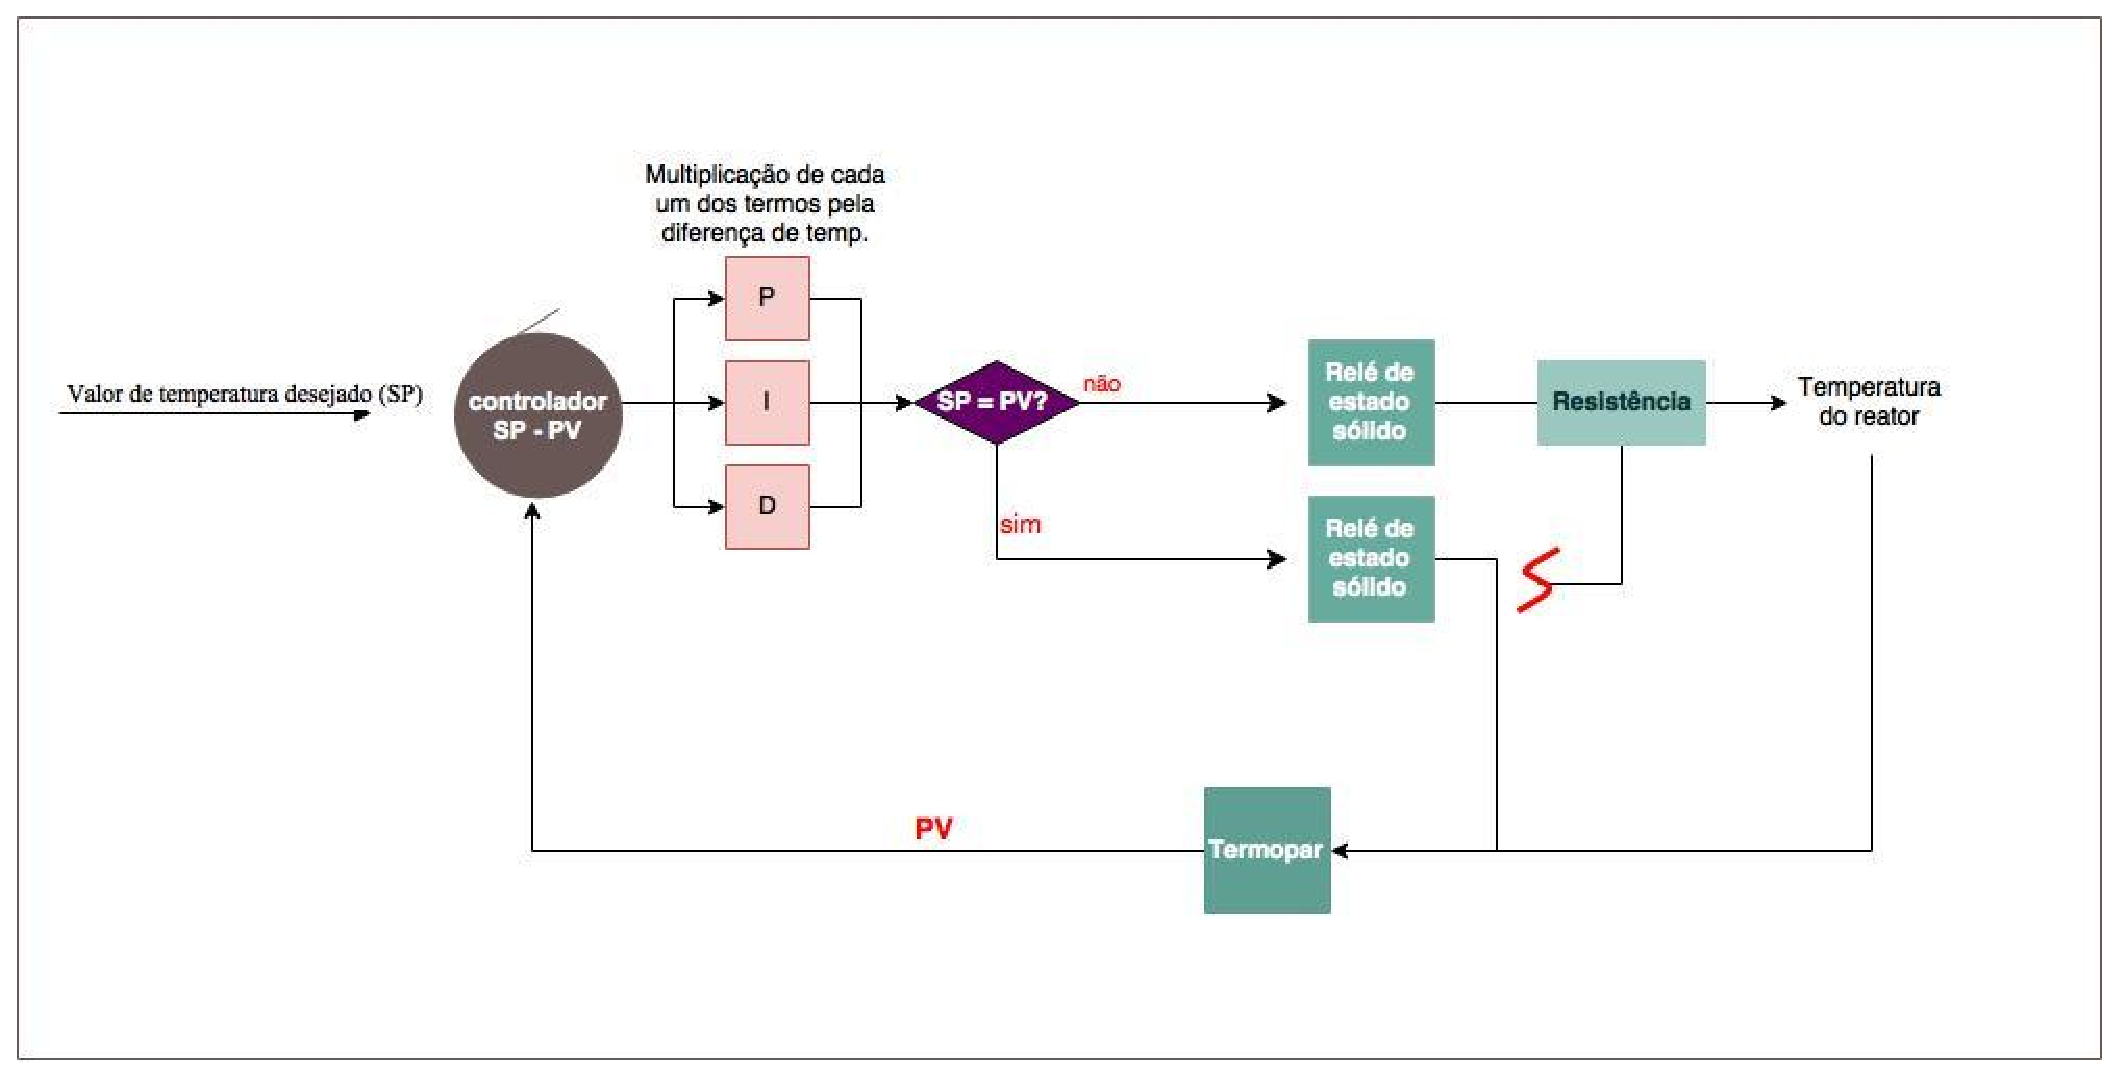
\includegraphics[keepaspectratio=true,scale=0.4]{figuras/processo.eps}
 \caption{Processor PID}
 \label{processo}
\end{figure}

Nesse projeto foi adquirido um controlador PID, junto com relé de estado sólido e um termopar, que foi validado controlando o aquecimento de uma lâmpada (Figura \ref{controlador}).

\begin{figure}[h]
 \centering
 \includegraphics[keepaspectratio=true,scale=0.2]{figuras/controlador.eps}
 \caption{Controlador}
 \label{controlador}
\end{figure}

\end{enumerate}

\subsection{Sistema de Refrigeração}

O sistema de refrigeração será composto por um reservatório abastecido com água da rede hidráulica convencional, onde, dentro de um sistema hermeticamente e termicamente isolado, será refrigerado por pastilhas peltier, mostrado na Figura \ref{refriferacao}.

\begin{figure}[h]
 \centering
 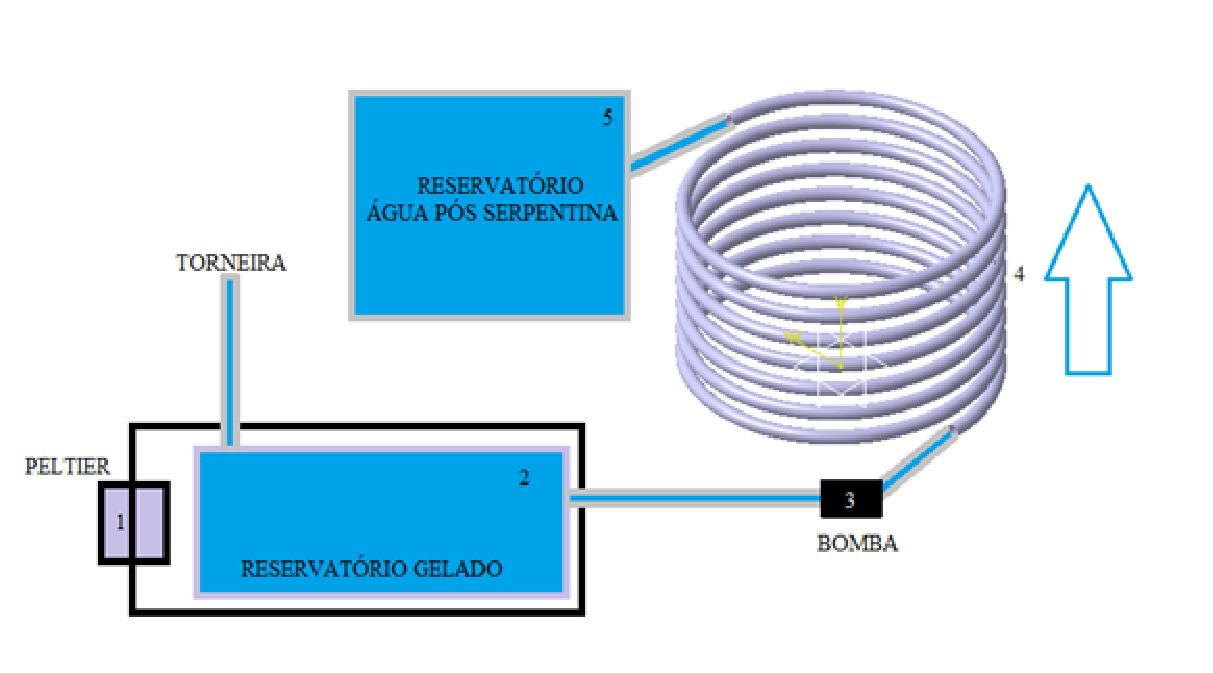
\includegraphics[keepaspectratio=true,scale=0.6]{figuras/refrigeracao.eps}
 \caption{Sistema de refrigeração}
 \label{refrigeracao}
\end{figure}


Este sistema será composto por cinco subsistemas, os quais serão descritos abaixo:

\begin{enumerate}
	\item \textbf{Pastilhas peltier + cooler}: Este subsistema será responsável pela refrigeração do reservatório gelado, serão instaladas duas placas peltiers ligadas a coolers e dissipadores que espalharão o ar gelado criado pelo lado frio da pastilha. As pastilhas peltier apresentaram eficiência de 10º C a menos em relação à temperatura ambiente, chegando a aproximadamente 6º C no lado frio. A Figura \ref{placa} mostra a formação de gelo no lado gelado da peltier.

	\begin{figure}[h]
	 \centering
	 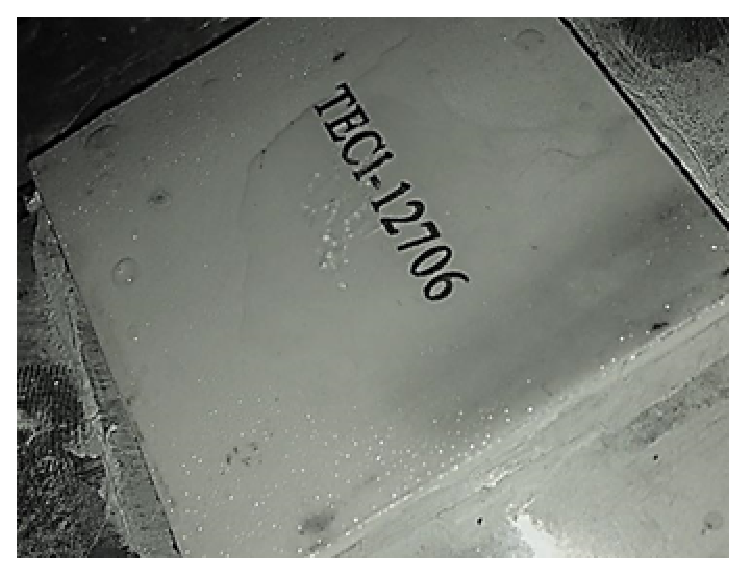
\includegraphics[keepaspectratio=true,scale=0.5]{figuras/placa.eps}
	 \caption{Placa peltier funcionando}
	 \label{placa}
	\end{figure}

	\item \textbf{Reservatório gelado}:	O reservatório gelado será feito com uma caixa térmica capaz de manter a temperatura gelada em seu interior. Dentro da caixa se encontrará uma serpentina de alumínio ou silicone que passará a água captada pela torneira, desta forma, a torneira será ligada no começo da reação e a água no interior da serpentina será resfriada pelo reservatório com as placas peltier, onde, a primeira vazão de água entrará na serpentina de resfriamento a uma temperatura menor do que a temperatura da água ambiente, auxiliando o resfriamento do líquido contido dentro do reator.

	\item \textbf{Bomba}: A bomba hidráulica terá a função de arrastar a água do reservatório gelado para dentro da serpentina que está no reator. A bomba também será responsável pela elevação da água desde que o fluxo entrará na parte de cima da tampa do reator seguindo diretamente para a extremidade inferior da serpentina que seguirá pelos tubos e sairá pela parte de cima, exemplificado na Figura X1. O equipamento utilizado será uma bomba DC 12 V, marca Javtop e modelo JT-600, para circulação de água quente ou fria. Sua vazão média é de 300 L/h, essa vazão será utilizada nos cálculos posteriores. A bomba utilizada é mostrada na Figura \ref{bomba}.

	\begin{figure}[h]
	 \centering
	 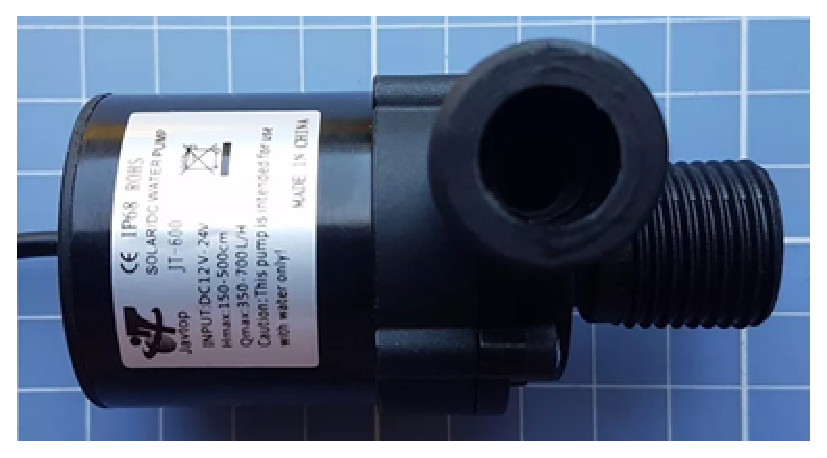
\includegraphics[keepaspectratio=true,scale=0.5]{figuras/bomba.eps}
	 \caption{Bomba Hidráulica DC}
	 \label{bomba}
	\end{figure}

	\item \textbf{Serpentina de resfriamento}: A serpentina, principal componente deste sistema, foi desenvolvida de acordo com os parâmetros métricos do reator. Os valores de diâmetro do tubo assim como as voltas dentro do reator foram selecionado a partir do produto disponível no mercado, considerando um passe de 1 cm em cada volta para que houvesse o fluxo de líquido com o impelidor. O diâmetro externo da serpentina foi escolhido considerando uma distância do impelidor para que não houvesse colisão entre as duas peças. A Figura \ref{serpentina2} mostra o esquema da serpentina assim como suas medidas.

	\begin{figure}[h]
	 \centering
	 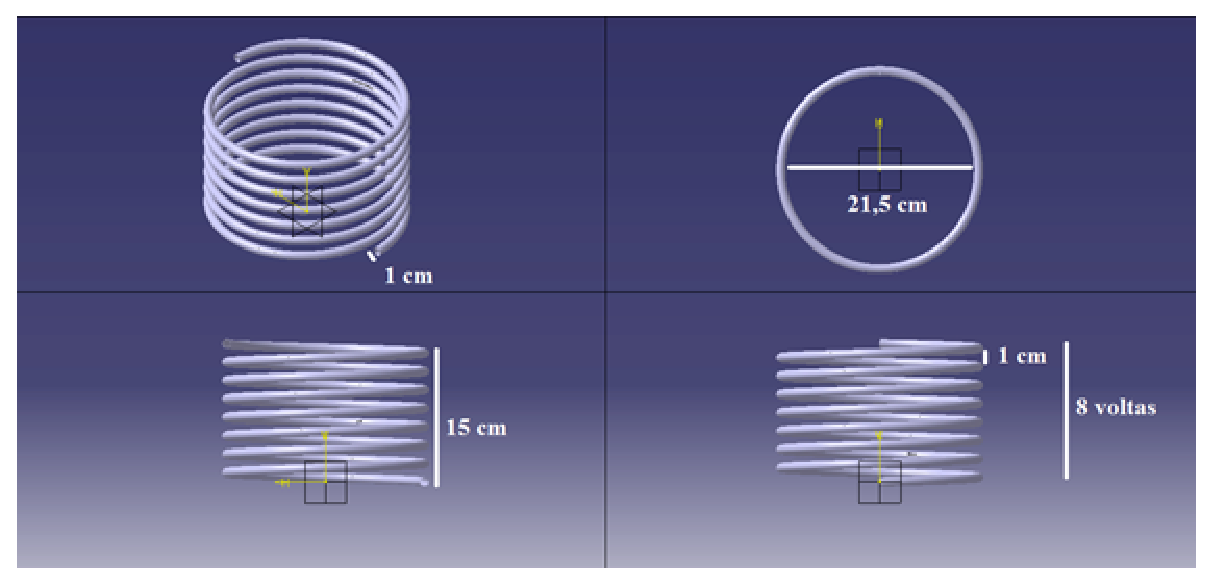
\includegraphics[keepaspectratio=true,scale=0.7]{figuras/serpentina2.eps}
	 \caption{Medidas da Serpentina}
	 \label{serpentina2}
	\end{figure}

Para o cálculo do tempo de resfriamento foi considerado o caso em que a água entre na serpentina em sua temperatura ambiente e o mosto em seu valor máximo de temperatura, observando o pior caso de resfriamento. Considerando o sistema acima, os seguintes parâmetros foram computados:

\begin{table}[h]
\centering
\begin{tabular}{|l|c|}
\hline
\multicolumn{1}{|c|}{Parâmetro}                     & Medida                                                        \\ \hline
Volume do mosto (V)                                 & 15 L                                                          \\ \hline
Diâmetro interno do tubo (d1)                       & 1 cm                                                          \\ \hline
Fluxo de água (W)                                   & 0,083 L \(s^{-1}\)									                          \\ \hline
Comprimento da serpentina submersa (L1)             & 12 m                                                          \\ \hline
Temperatura inicial do mosto (t1)                   & 60º C                                                         \\ \hline
Temperatura final desejada do mosto (t2)            & 30º C                                                         \\ \hline
Calor específico do mosto (Cm)                      & 3100 J \(kg^{-1} K^{-1}\) 																		\\ \hline
Densidade do mosto (D)                              & 1,065 g \(cm^{3-1}\)                      									  \\ \hline
Calor específico da água (Cj)                       & 4187 J \(kg^{-1}\) \(K^{-1}\) 																		\\ \hline
Regime do fluxo                                     & Intermitente                                                  \\ \hline
Coeficiente Global de transferência de calor (U) ** & 500 W \(m^{2-1} k^{-1}\)      																		\\ \hline
Densidade da água de resfriamento                   & 0,998 g \(cm^{3-1}\)                        									\\ \hline
Temperatura de entrada da água (T)                  & 27 ºC                                                         \\ \hline
\end{tabular}
\caption{Tempo de resfriamento}
\label{resfriamento}
\end{table}

** O valor do coeficiente global foi considerado a partir de coeficientes globais gerais encontrados na literatura. Para este trabalho foi considerado o seguinte coeficiente: Líquido Forçado (fluxo) Água – Líquido livre de convecção : 500 - 1500 W/m2K (serpentina de resfriamento- espiral).

Calculando a massa do mosto:
\[m =  D \cdot V = 1,065 \cdot 15000 = 15,98 Kg\]

O calor que terá que ser removido pela serpentina:
\[Q = m \cdot Cm \cdot (t2 - t1) = 15,98 \cdot 3100 \cdot (30-60) = -1488,14 KJ\]

A área da serpentina:
\[A = \pi \dot d1 \cdot L1 = \pi \cdot 0,01 \cdot 12 = 0,377 m^2\]

Desta forma, o tempo estimado de resfriamento, a partir dos dados anteriores e considerando um regime intermitente será dado pela seguinte fórmula:

\[t = \frac{\ln\frac{(T-t_{1})}{(T-t_{2})}}{\frac{C_{j}\cdot W}{C_{m}\cdot m}}\cdot\frac{\exp(\frac{U\cdot A}{C_{j}\cdot W})}{\exp(\frac{U\cdot A}{C_{j}\cdot W}) - 1}\cdot\frac{1}{60s} = \frac{\ln\frac{(27-60)}{(27-30}}{\frac{4187\cdot 0,083}{3100\cdot 15,98}}\cdot\frac{\exp(\frac{500\cdot 0,377}{4187\cdot 0,083})}{\exp(\frac{500\cdot 0,377}{4187\cdot 0,083}) - 1}\cdot\frac{1}{60s} \cong 13,6 \min\]

Assim, com essas condições, o mosto demoraria cerca de 14 minutos para resfriar de 60º para 30º C com uma serpentina imersa no líquido. Os cálculos são aproximados e alguns erros estão embutidos, desta forma, trabalharemos com 15 min.

Por fim, calcula-se a quantidade de água necessária para um ciclo de resfriamento de cerca de 30 ºC:

\[V_{necessário}=W.t.60\]
\[V_{necessário}=0,083  \cdot 15  \cdot 60 \cong  75 L\]

Portanto, para este sistema de resfriamento, 75 L de água a temperatura ambiente serão necessários para abaixar a temperatura em 30 ºC em aproximadamente 15 minutos.

	\item \textbf{Reservatório de água pós serpentina}: O reservatório de água que recolherá a água após passar por dentro da serpentina servirá para que o processo não perca eficiência, de forma a captar a água quente advinda da serpentina e guardá-la até a próxima reação. Este tanque será ligado a torneira, ligação essa que ficará fechada durante a fermentação, desta forma, quando a reação acabar, pode-se abrir a ligação e deixar o escoamento acontecer tanto por meio deste reservatório quanto da rede hidráulica para o recomeço de uma nova reação. Este reservatório permite também que se utilize somente a água da rede hidráulica.

\end{enumerate}

\subsection{Dimensionamento da Pressão Interna}

Durante o processo de fermentação ocorre a formação de gás carbônico, e devido ao fato do reator ser vedado é importante que se calcule a quantidade de gás formado bem como a pressão interna dele.

Para o cálculo foram feitas algumas considerações:

\begin{itemize}
	\item temperatura constante
	\item não há dissolução de \(CO_{2}\) na fase líquida
	\item não há transferência de massa entre a fase líquida e gasosa
	\item \(CO_{2}\) considerado gás ideal
	\item Conversão de 100\% do açúcar em álcool
	\item Teor de sólidos solúveis do mosto = 18ºBrix
	\item mosto obtido a partir caldo de cana
\end{itemize}

Primeiramente foi feito o cálculo considerando que não haveria escape de gás a fim de verificar a necessidade do sistema de captação de \(CO_{2}\). A tabela abaixo mostra alguns dados iniciais para os cálculos:

\begin{table}[h]
\centering
\begin{tabular}{|l|l|}
\hline
\multicolumn{2}{|l|}{Dados} \\ \hline
\(\rho_{cana}[gL^{-1}]\)             &    1041,3          \\ \hline
\(V_{mosto}\)             &      20,85        \\ \hline
\(V_{gás}\)             &     8,3         \\ \hline
T [K]             &       303       \\ \hline
R\(atm.L.mol^{-1}.K^{-1}\)             &  0,082            \\ \hline
\(mm_{CO_2}g.mol^{-1}\)             &     44         \\ \hline
\(mm_{glicose}g.mol^{-1}\)         &    180          \\ \hline
\end{tabular}
\caption{Dados iniciais}
\label{dados-iniciais}
\end{table}


A densidade do caldo da cana foi calculado experimentalmente, e a partir dela, é possível saber a massa de mosto:

\[m=\rho.V\]
\[m = 1041,3 \times 20,85\]
\[m = 21.711,1 g\]

A definição de ºBrix é que a cada 1g de açúcar em 100g de mosto, se eleva 1ºBrix. Dessa forma é possível calcular a massa de açúcar que será consumida durante a reação, sabendo que para conversão de 100\% seriam consumidos o equivalente à 18ºBrix. Dessa forma se tem a relação:

\[18g \,de\, açúcar \rightarrow 100g \,de\, mosto\]

\[3.907,99 g \,de\, açúcar \rightarrow 21.711,1 g \,de\, mosto\]

Para saber a massa de gás que é produzida, é necessário fazer a relação estequiométrica da reação de fermentação:

\[C_{6}H_{12}O_{6}\rightarrow 2CO_{2}\]

Ou seja, para cada mol de açúcar consumido são produzidos 2 mol de gás carbônico. Assim, pode se relacionar as massas molares da glicose e do dióxido de carbono:

\[180 g \,de\, C6H12O6 \rightarrow (2x44) g \,de\, CO_{2}\]

\[3.907g \,de\, C6H12O6 \rightarrow 1.910,58 g \,de\, (CO_{2}\]

Desta forma, é possível calcular a pressão a partir da lei dos gases:
\[PV = nRT\]

Onde:

\begin{itemize}
	\item P: pressão
	\item V: volume
	\item n: número de mol
	\item R: Constante universal dos gases
	\item T: temperatura
\end{itemize}

O número de mol pode ser dado em função da massa e da massa molar do gás:

\[P = \frac{m.R.T}{mm.V}\]

\[P = \frac{1910,58 .0,082.301 }{44.8,3}\]

\[P = 129,13 atm\]


Apesar de elevado, tal valor é justificado pelo volume de mosto, e principalmente por se considerar o caso extremo em que toda açúcar seria fermentada, sendo que em casos reais cerca de apenas (40 a 50)\% são realmente convertidos. É importante ressaltar também que esse é o valor é considerado para o reator sem escape de gás e ocupando apenas o volume não ocupado pelo mosto. Ainda sim, foi avaliado que é necessário uma válvula de escape para o gás, e devido ao grande aumento pressão que ocorre na reação foi desconsiderado o sistema para captar \(CO_{2}\), uma vez que por questão de segurança é mais viável que apenas seja feito um sistema de escape e não de captação.

A segunda abordagem foi feita considerando a área da secção transversal para escape do gás sem atrito, onde foi calculada a taxa de formação e de saída dele, e a partir disso a pressão que permanece dentro do reator.

Essa modelagem foi feita baseada no estudo de Romanholi et al. (2009)  que calculou a pressão remanescente em um fermentador variando o tamanho do orifício de saída de o volume de mosto. Primeiramente, é feito o balanço de massa para o \(CO_{2}\) considerando apenas o volume vazio, sem mosto.

\[\frac{dn_{CO_2}}{dt} = r_{CO_2}\cdot V_{caldo}-G\]

Onde:

\begin{itemize}
	\item \(r_{CO_2}\) : velocidade de formação do  \(CO_{2}\) \([mol.L^{-1} \cdot h^{-1}]\)
	\item G': vazão de saída de gás \([mol.h^{-1}]\)
\end{itemize}

Sendo que essa vazão é dada em função do fluxo mássico (G), da área do orifício de saída \((A_{orifício})\), e da pressão interna e externa, obtidos a partir do balanço de energia e massa:

\[G = P_{0}.\sqrt{\frac{K.mm}{R.T_{0}}}.\frac{M_{1}}{(1+\frac{K-1}{2}.M_1^2)^{\frac{K+1}{2(k-1)}}}[ \frac{Kg}{m^{2}.s}]\]

Em que ‘k’ é relação entre os calores específicos do fluido nas fases líquida e gasosa, para o \(CO_{2}\)  é  1,288. \(M_{1}\) é o número de Mach na garganta do orifício, que apresenta valor unitário uma vez que o fluxo de saída não é subsônico. \(P_{0}\) é a pressão inicial dentro do reator, considerada como 1 atm. E o diâmetro de saída de 23 mm. Assim, a vazão de saída de gás é dada por:

\[G'=\frac{G.A_{orifício}}{mm}\]

Substituindo todos os valores, se tem:

\[G = 89,69 [g.m^{-2}.s^{-1}]\]
\[G’ = 0,00085 [mol.s^{-1}]\]

A partir da lei universal dos gases ideais se tem:

\[PV = nRT\]

Diferenciando essa equação, se tem dois parâmetros que variam em função do tempo, a pressão e o número de mols, já que a medida que o açúcar vai sendo  consumido, o número de mols de gás carbônico vai aumentando conforme ele vai sendo produzido, e por ser um sistema com volume fixo, a pressão tende a aumentar também. Dessa forma, a variação da pressão interna no reator pode ser obtida a partir da equação diferencial abaixo:

\[\frac{dP}{dt}=\frac{dn}{dt}.\frac{R.T}{V_{gás}}\]

Uma vez que uma equação diferencial depende da outra, elas foram resolvidas simultaneamente de forma numérica a partir do método Runge-Kutta de 4ª ordem utilizando Microsoft Excel. Foram simulados valores considerando o tempo de duração de 24h. Dos valores obtidos, foram selecionados e os 15 maiores valores da pressão formada e da pressão que sai do reator para compilação gráfica e análise, sendo que os maiores valores são referentes aos maiores tempo de reação.

\begin{figure}[H]
 \centering
 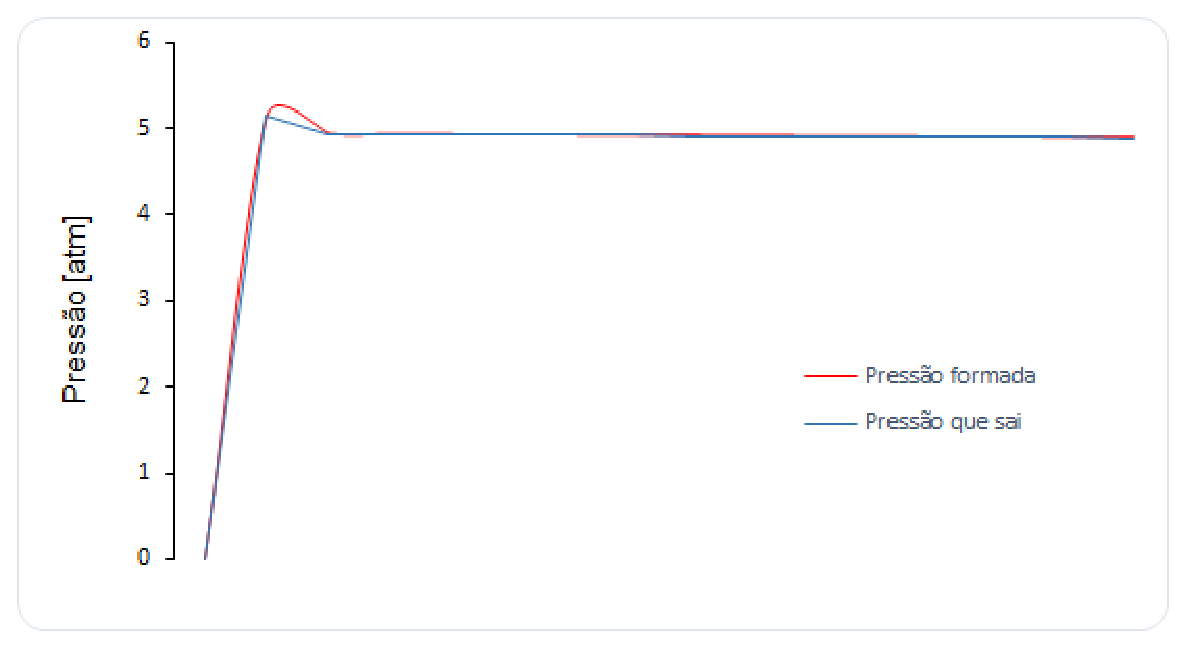
\includegraphics[keepaspectratio=true,scale=0.5]{figuras/pressao.eps}
 \caption{Comportamento da Pressão}
 \label{pressao}
\end{figure}

Uma vez que uma equação diferencial depende da outra, elas foram resolvidas simultaneamente de forma numérica a partir do método Runge-Kutta de 4ª ordem utilizando Microsoft Excel. Foram simulados valores considerando o tempo de duração de 24h. Dos valores obtidos, foram selecionados e os 15 maiores valores da pressão formada e da pressão que sai do reator para compilação gráfica e análise, sendo que os maiores valores são referentes aos maiores tempo de reação.

\begin{figure}[h]
 \centering
 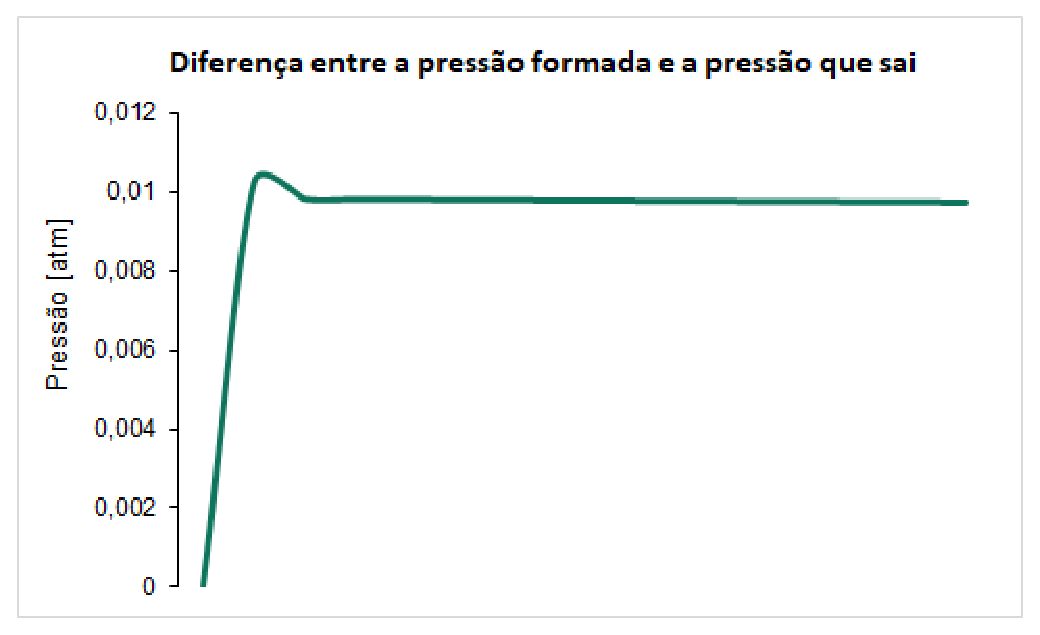
\includegraphics[keepaspectratio=true,scale=0.5]{figuras/pressao2.eps}
 \caption{Diferença da Pressão}
 \label{pressao2}
\end{figure}

A partir dos valores obtidos, é possível observar que a pressão interna tende a se estabilizar e assim, é possível afirmar que o diâmetro do orifício de saída do gás, bem como o volume disponível para formação do \(CO_{2}\)  satisfazem as condições de reação.

\subsection{Circuito elétrico do Sistema}

O circuito foi projetado levando em conta os componentes do sistema de aquecimento e refrigeração. O sistema de aquecimento é alimentado em 220V corrente alternada, enquanto o de refrigeração é alimentado em 12V, de forma que foi colocado uma fonte chaveada para fornecer essa tensão necessária. A figura a seguir representa o esquema do circuito, onde D1, D2 e D3 são disjuntores.

\begin{figure}[h]
 \centering
 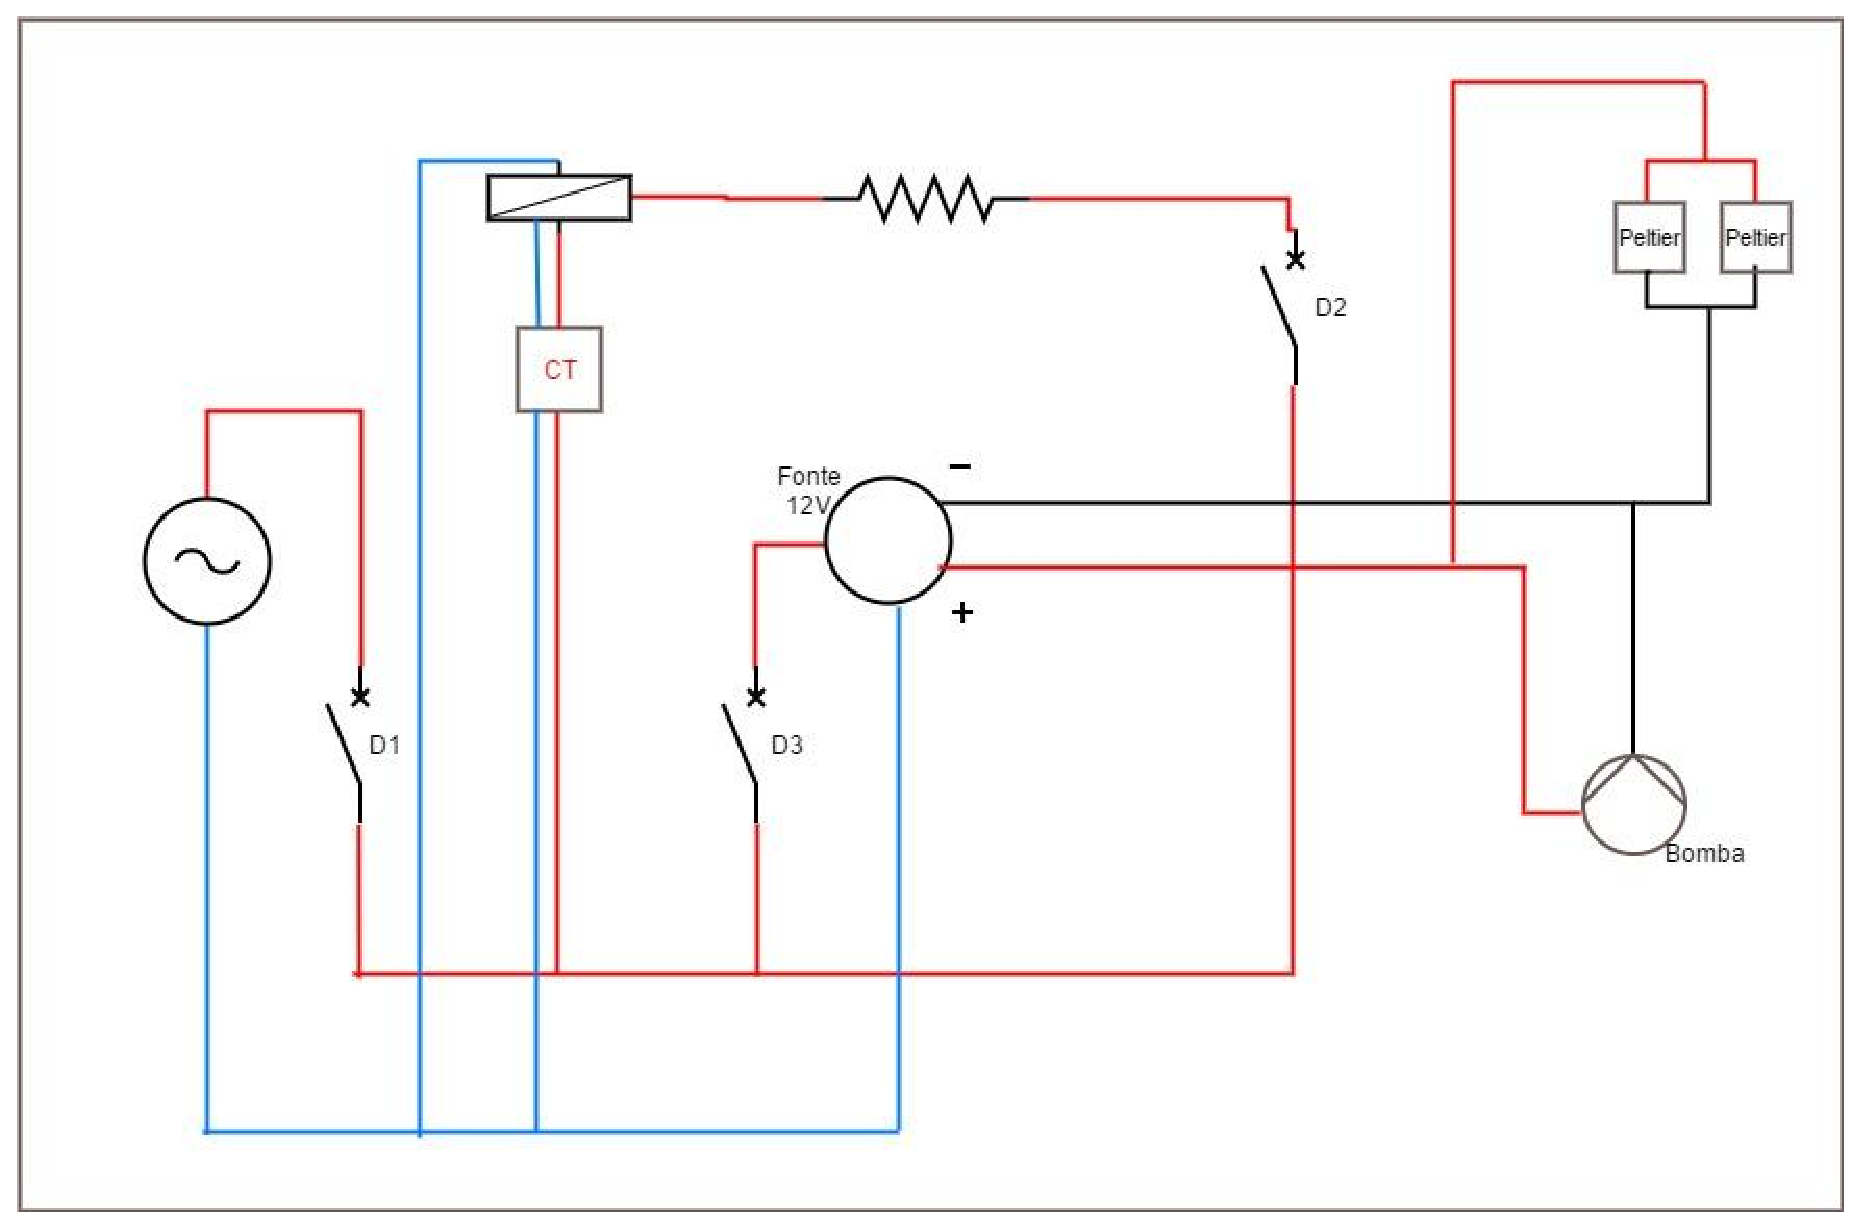
\includegraphics[keepaspectratio=true,scale=0.4]{figuras/circuito.eps}
 \caption{Circuito Elétrico do Sistema}
 \label{circuito}
\end{figure}

\subsection{Fabricação estrutural e componentes}

As dimensões do biorreator foram determinadas de acordo com a requisitos impostos a partir do subgrupo de eletrônica, de energia e para melhoria de alguns parâmetros do sistema de agitação.

Para determinação da altura do biorreator foi levado em consideração que os sensores de pressão, conforme passado pelo subgrupo da eletrônica, deveriam estar separados em um distância perpendicular de 250 mm e ambos imersos em líquido. Para completar, o subgrupo de energia determinou que o volume ocupado pelo líquido deveria ser de 70\% do volume total do tanque, resultando assim, em uma altura total de 450 mm. O diâmetro selecionado foi aquele fabricável que mais se ajustou ao sistema de agitação sendo esse com valor de 310 mm. A figura abaixo ilustra essas medidas do tanque.

\begin{figure}[h]
 \centering
 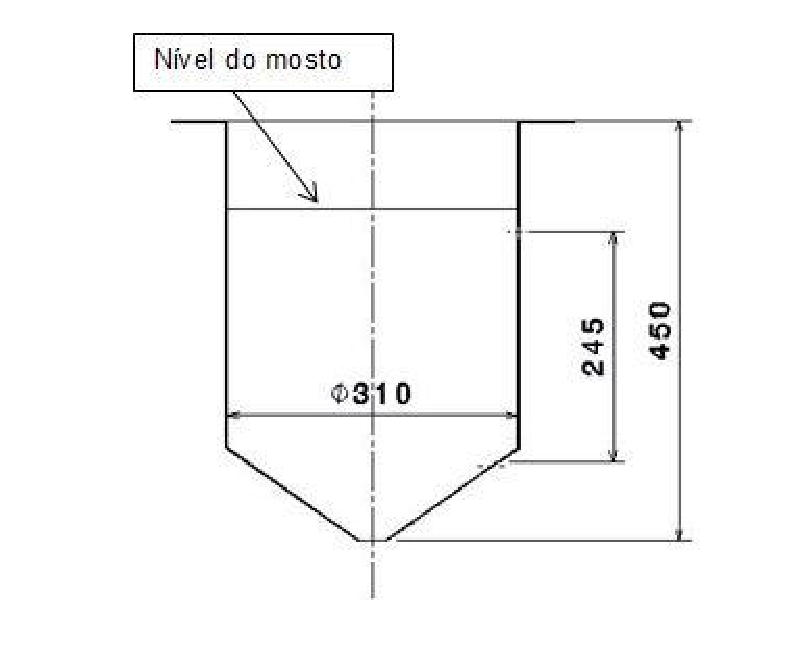
\includegraphics[keepaspectratio=true,scale=0.5]{figuras/nivel.eps}
 \caption{Posicionamento dos sensores de pressão}
 \label{nivel}
\end{figure}

A figura abaixo mostra o tanque do biorreator em produção, após o processo de soldagem.

\begin{figure}[h]
 \centering
 \includegraphics[keepaspectratio=true,scale=0.2]{figuras/soldagem.eps}
 \caption{Biorreator após soldagem}
 \label{soldagem}
\end{figure}

\subsubsection{Cálculo analítico das tensões no Biorreator}

De acordo com os cálculos realizados previamente, os valores de pressão interna no tanque após a colocação do duto de escape do CO2 serão muito baixos. Porém por uma questão de segurança, serão calculadas as tensões no tanque para valores de pressão que vão até o para atuação da válvula de segurança de pressão.

Segundo (Iecker, 2014), as equações que regem os valores de tensão em paredes cilíndricas, tampo cônico e tampos planos são:

Tensões no cilíndro:
\[S = (\frac{P.R}{t}+0,6P). \frac{1}{E}\]

Onde:

\begin{itemize}
	\item P = pressão [KPa];
	\item R = Raio;
	\item t = espessura;
	\item E = eficiência da junta.
\end{itemize}

Tensões em tampo cônico:
\[S = \left(\frac{P.R}{t.cos\alpha}+0,6P\right). \frac{1}{E}\]

Onde:
\begin{itemize}
	\item \(\alpha\) = ângulo do cone
\end{itemize}

Tensões em tampos planos:
\[S=N.P.\left(\frac{D}{t}\right)^2\]

Onde:
\begin{itemize}
	\item D = diâmetro da flange;
	\item N = 0,3 com flange para união aparafusada.
\end{itemize}

Na condição onde a pressão chegar a máxima para abertura da válvula de segurança.

\subsubsection{Dimensionamento das colunas para sustentação}

Para uma melhor ergonomia na hora de manusear o biorreator foi determinado a implementação de colunas de sustentação para prover uma maior comodidade ao usuário.

A altura determinada para as colunas é de 540 mm de modo a fazer com que o biorreator possua uma altura total de 0,95 m. Altura essa que foi verificada para atender o percentil 50 de altura da população feminina do brasileira. A figura abaixo mostra as dimensões do conjunto.

\begin{figure}[h]
 \centering
 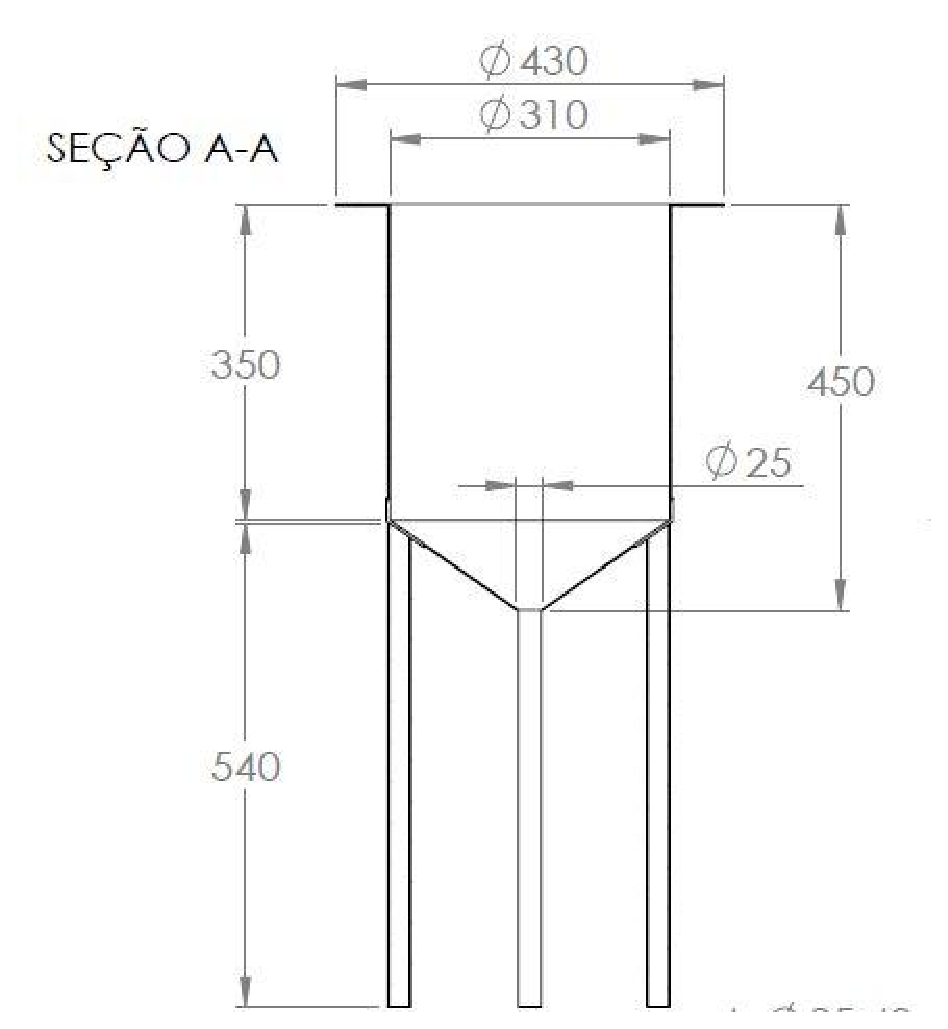
\includegraphics[keepaspectratio=true,scale=0.5]{figuras/tanque.eps}
 \caption{Tanque com as Colunas}
 \label{tanque}
\end{figure}


Após a determinação da altura das colunas deve-se então verificar um perfil que atenda as solicitações de esforços. Foram selecionados três tubos de inox 304 com diâmetro externo de 1””

Foi realizada uma verificação da possibilidade de flambagem dos apoios do biorreator.

O biorreator possui diversas finalidades, dentre elas aferir temperatura e pressão, além de sistemas de resfriamento e aquecimento. Para todos, foram estabelecidos os locais específicos de perfuração através de um gabarito impresso em escala real para dar precisão. Para o dreno na parte inferior do tanque, há uma válvula de esfera que viabiliza a remoção de levedura, assim como uma válvula na lateral da estrutura para retirar amostras da mistura. Essas regiões foram soldadas com tubo inoxidável de 1 polegada cada.

\begin{figure}[h]
 \centering
 \includegraphics[keepaspectratio=true,scale=0.3]{figuras/valvula.eps}
 \caption{Tanque com as Colunas}
 \label{valvula}
\end{figure}

O sensor de temperatura depende de uma estrutura que está em desenvolvimento, onde haverá um orifício para inserção vedado com uma o’\textit{ring} e pressionado através de uma rosca.

Um elemento essencial para o sistema de fermentação, devido à alta quantidade de emissão de gás carbônico é o manômetro, combinado a uma válvula de alívio de pressão

\begin{figure}[h]
 \centering
 \includegraphics[keepaspectratio=true,scale=0.4]{figuras/manometro.eps}
 \caption{Válvula de alívio de pressão}
 \label{manometro}
\end{figure}

\begin{figure}[h]
 \centering
 \includegraphics[keepaspectratio=true,scale=0.4]{figuras/alivio.eps}
 \caption{Manômetro de pressão de ar}
 \label{alivio}
\end{figure}

O diagrama para o projeto no que tange ao cálculo de tensões e validação está expresso a seguir.

\begin{figure}[h]
 \centering
 \includegraphics[keepaspectratio=true,scale=0.5]{figuras/diagrama.eps}
 \caption{Diagrama do projeto do Biorreator}
 \label{diagrama}
\end{figure}

\subsection{Dimensionamento do Sistema de Agitação}

De acordo com (Barbosa, 2004), o sistema de agitação tem como objetivo promover uma melhor circulação do fluido por todo o volume do tanque. Alguns parâmetros de agitação são essenciais para que haja um bom funcionamento e eficiência.

Parâmetros como os tipos de pás, diâmetro do impelidor, dimensões do tanque, altura do fluido no tanque, viscosidade, densidade do fluido e rotação dos impelidores são responsáveis pelo dimensionamento desse sistema (BARBOSA, 2014).

Segundo Barbosa (2014), as pás do tipo retas a 90º criam um fluxo radial e promovem uma boa uniformização da mistura em fluidos pouco viscosos. Esse será então o tipo de impelidor a ser adotado no projeto do sistema de agitação.

De acordo com (McCabe, 1981), o valor do diâmetro do impelidor (Da) é dado por:

\[D_{a}=\frac{1}{3}.T\]
\[D_{a}=\frac{1}{3}.310 = 103mm\]

Onde:
\begin{itemize}
	\item T = Diâmetro do tanque.
\end{itemize}

A altura (w) das pás são calculadas de acordo com a equação abaixo:
\[w = \frac{1}{5}Da\]
\[w = 20,6 mm\]

De acordo com (FASANO et al 1994), a quantidade de impelidores que o tanque deve possuir depende da razão entre a altura do líquido (Z) e o diâmetro do tanque (T), além do número de Reynolds. O quadro 1 mostra o número de impelidores de acordo com Z/T e a faixa do número de Reynolds.

\begin{table}[]
\centering
\resizebox{\textwidth}{!} {
\begin{tabular}{|c|c|c|c|c|c|c|}
\hline
\multicolumn{7}{|c|}{Valores máximos permitidos Z/T}                                                                                                                                           \\ \hline
\multicolumn{1}{|l|}{Faixa de Re} & \multicolumn{2}{l|}{Impelidor alta eficiência} & \multicolumn{2}{l|}{Impelidor 4 pás 45º} & \multicolumn{2}{l|}{Impelidor 4 pás planas ou 6 pás (Rushton)} \\ \hline
\multicolumn{1}{|l|}{}            & Único                  & Duplo                 & Único               & Duplo              & Único                          & Duplo                         \\ \hline
10 - 100                          & 0,9                    & 1,7                   & 0,8                 & 1,5                & 0,6                            & 1,2                           \\ \hline
100 - 1000                        & 1,3                    & 2,1                   & 0,9                 & 1,6                & 0,6                            & 1,2                           \\ \hline
1000 - 10000                      & 1,4                    & 2,3                   & 1,1                 & 1,8                & 0,7                            & 1,4                           \\ \hline
\textgreater 10000                & 1,5                    & 2,4                   & 1,2                 & 1,9                & 0,8                            & 1,6                           \\ \hline
\end{tabular}
}
\caption{Determinação da quantidade de impelidores.(FASANO et al 1994)}
\label{impelidores}
\end{table}

\subsubsection{Cálculo do diâmetro do eixo}

Segundo (Barbosa, 2014), o dimensionamento do eixo do agitador é feito após ser calculado o valor de potência e torque consumidos pelo sistema de agitação.

\subsubsubsection{Potência Consumida}

Para a realização do cálculo da potência consumida necessita-se do valor do número de Reynolds que é dado pela equação a seguir (BARBOSA, 2014).
\[Re = \frac{\rho.n.D_{a}^2}{\mu}\]

Onde:

\begin{itemize}
	\item \(\rho\) = densidade do fluido [Kg/m3];
	\item n = frequência de rotação [rps];
	\item \(\mu\) = viscosidade dinâmica.
\end{itemize}

A densidade e a viscosidade da mistura mosto mais leveduras foram obtidas de forma experimental através de ensaios no laboratório de Química experimental da FGA no Galpão. Os ensaios foram realizados com o mosto na temperatura de 31 ºC, simulando assim as condições de fermentação no biorreator. A FIGURA \ref{equipamentos} mostra algumas etapas da realização do experimento.

\begin{figure}[h]
 \centering
 \includegraphics[keepaspectratio=true,scale=0.4]{figuras/equipamentos.eps}
 \caption{Realização do experimento}
 \label{equipamentos}
\end{figure}

A viscosidade cinemática (\(\upsilon\)) da mistura foi obtida com o auxílio de um viscosímetro e seu valor encontrado foi de 2,879 cts.
A densidade foi obtida através da mensuração com o auxílio de uma balança de precisão da massa do mosto de um volume. Para cada litro de caldo de cana foram usadas 10g de leveduras. O valor de densidade da mistura é de 1065,51 \(Kg/m^3\).

O valor da viscosidade dinâmica pode então ser calculada através da Equação abaixo:

\[\mu=\rho.\upsilon = 0,0030670 \frac{Kg}{m.s}\]

O valor da potência de agitação (Nm) é obtido através da equação 5 (BARBOSA, 2014).

\[N_{m}=N_{p_0}.\rho.D_a^5.n^{3}\]

\[N_{p}=f(Re)\]

Onde:
\begin{itemize}
	\item Np = Número de potência
\end{itemize}

O número de potência está associado ao número de Reynolds. Seu valor para turbinas de pás retas é determinado através do gráfico Npo X Re mostrado na FIGURA X3.

\begin{figure}[h]
 \centering
 \includegraphics[keepaspectratio=true,scale=0.5]{figuras/potencia.eps}
 \caption{Escolha do número de potência.}
 \label{potencia}
\end{figure}

Para saber a potência de agitação efetiva \((N_{me})\) é necessário levar em consideração a eficiência do rolamento \((\eta_{r})\), e a eficiência de acionamento \(()\eta_{a})\) devido ao uso do selo mecânico. Os valores de \((\eta_{r})\) e \((\eta_{a})\) são 0,98 e 0,85, respectivamente. A equação 6 dá o valor de Nme (BARBOSA, 2014).

\[N_{me}=\frac{N_{m}}{\eta_r.\eta_a}\]

\subsubsubsection{Dimensionamento do eixo}

O cálculo do eixo é feito para solicitações de torção e flexão combinadas. Esse tipo de eixo só teria esforços cíclicos se houver um valor de desbalanceamento residual alto. (SHIGLEY, 2005 )

Tendo calculado a potência efetiva de agitação e de posse da velocidade de rotação é possível então determinar o torque requerido que atua sobre o eixo. O torque é calculado de acordo com a equação abaixo. (BARBOSA, 2004).

\[T=\frac{N_{me}}{2\pi.n}\]

Considerando a condição mais crítica no agitador onde há um travamento no eixo a força desenvolvida (\(F_f\)) é dada pela equação: (BARBOSA, 2004).

\[F_f=\frac{T}{0,75R}\]

Onde:

\begin{itemize}
	\item R = raio do impelidor
\end{itemize}

O momento fletor (Mf) causado no eixo é calculado de acordo com a equação abaixo (BARBOSA, 2004)

\[M_{f}=F_{f}.l\]

Onde:
\begin{itemize}
	\item l = comprimento em balanço do eixo.
\end{itemize}

O diâmetro do eixo pode ser calculado então pela equação de Von Mises a seguir (SHIGLEY, 2005).

\[d=\left[\left(\frac{16.n_s}{\pi.S_y}\right).\left(4Mf^2+\frac{3T^2}{4}\right)^\frac{1}{2}\right]^\frac{1}{3}\]

Onde:
\begin{itemize}
	\item \(n_{s}\) = fator de segurança;
	\item \(S_{y}\) = tensão de escoamento do material (240 MPa para o inox 304)
\end{itemize}

As equações foram implementadas no MATLAB e seu código está presente no anexo A. A metodologia adotada para o funcionamento do código mostrando as entradas e saídas são mostradas no diagrama abaixo.

\begin{figure}[h]
 \centering
 \includegraphics[keepaspectratio=true,scale=0.4]{figuras/blocos.eps}
 \caption{Diagrama de blocos com sequência adotada em MatLab.}
 \label{blocos}
\end{figure}

Os valores obtidos pela rotina de dimensionamento no MATLAB foram comparados com valores obtidos por um software de agitação e mistura comercial chamado cerebromix 10.1 a fim da validação da rotina. O software foi usado em sua versão Demo que é disponibilizada gratuitamente.

Os mesmos parâmetros de entrada do programa de agitação foram inseridos no código de MATLAB e os resultados apresentados por ambos serão mostrados na tabela 1.
